\chapter{Implementation}
\label{chap:implementation}

In this chapter, we will go through our \emph{application generator}, explaining in detail how it works and how it is implemented under the hood. We will focus both on the \emph{platform} aspect and the \emph{framework} aspect. As for the \emph{platform} aspect, we will show how a non-developer can use the new \emph{platform} to generate and share Linked Data based applications. As for the \emph{framework} aspect, we will provide a potential developer with a step-by-step guide for how to implement a new \emph{visualizer}. As our generator is built on top of LinkedPipes Visualization, its official name is LinkedPipes Application Generator. For brevity, we will refer to it simply as to (our) \emph{application generator}.

Note that certain sections of this chapter, especially the step-by-step guide, are very technical and rather exhaustive. Under normal circumstances those sections would be part of the separate development guide. Nevertheless, as one of the goals of this thesis was to develop a framework, we need to convince the reader that we fulfilled this goal. We can only do that by providing enough detail about how the framework works and especially how it can be used by other developers.

\section{Overview}

Before we dive into technical details, let us walk the reader through the \emph{application generator} features from a user perspective. We will start by describing a sample use case scenario and then we will continue with individual \emph{platform} features.

\subsection{Sample use case scenario}
\label{sec:implementation:use-case-scenario}

In this scenario, we will utilize the D3.js Chord Visualizer and the Asylum Seekers 2015 data set. Both will be properly described later in a separate chapter dedicated to this particular visualizer. Let us say that our fictional user is a journalist writing an article on the refugee crisis. He comes across our \emph{application generator} and finds there the Asylum Seekers 2015 data set. The Figures \ref{fig:scenario-01-browse-data-sources} to \ref{fig:scenario-11-embedded-application} show step-by-step how the journalist can use our tool to create an interactive application and share it with his readers. 

The actual mechanics of this visualizer will be explained later in the aforementioned separate chapter. Nevertheless, on a more general level this scenario nicely illustrates the principles that we suggested in the system proposal (Section \ref{sec:proposal:features}). 

\begin{itemize}
\item \emph{Data analysis}. The selected data set is automatically \emph{analyzed} and an appropriate visualization is offered to the user (Figure \ref{fig:scenario-02-discovery-result}).
\item \emph{Configuration}. The configuration phase allows the user to work with the data and to affect the final shape of the application before it gets published.  He can select for the visualization only the data he (or his audience) is interested in (Figure \ref{fig:scenario-05-search-graph}). He can even extend the data set itself with missing information (Figure \ref{fig:scenario-08-custom-label-editor}). 
\item \emph{Online sharing}. The application can be easily shared using its public URL (Figure~\ref{fig:scenario-09-published-app}).
\item \emph{Non-developers friendly}. None of these steps require any advanced programming knowledge. The only exception in this case is the preparation of the data set. Unfortunately, the original data are not available in RDF and the conversion has to be done by an expert. Nevertheless, once the data set is prepared and available in the \emph{application generator}, it can become a source for a large number of different applications (the \emph{platform} feature.
\end{itemize}
\begin{figure}
	\centering
	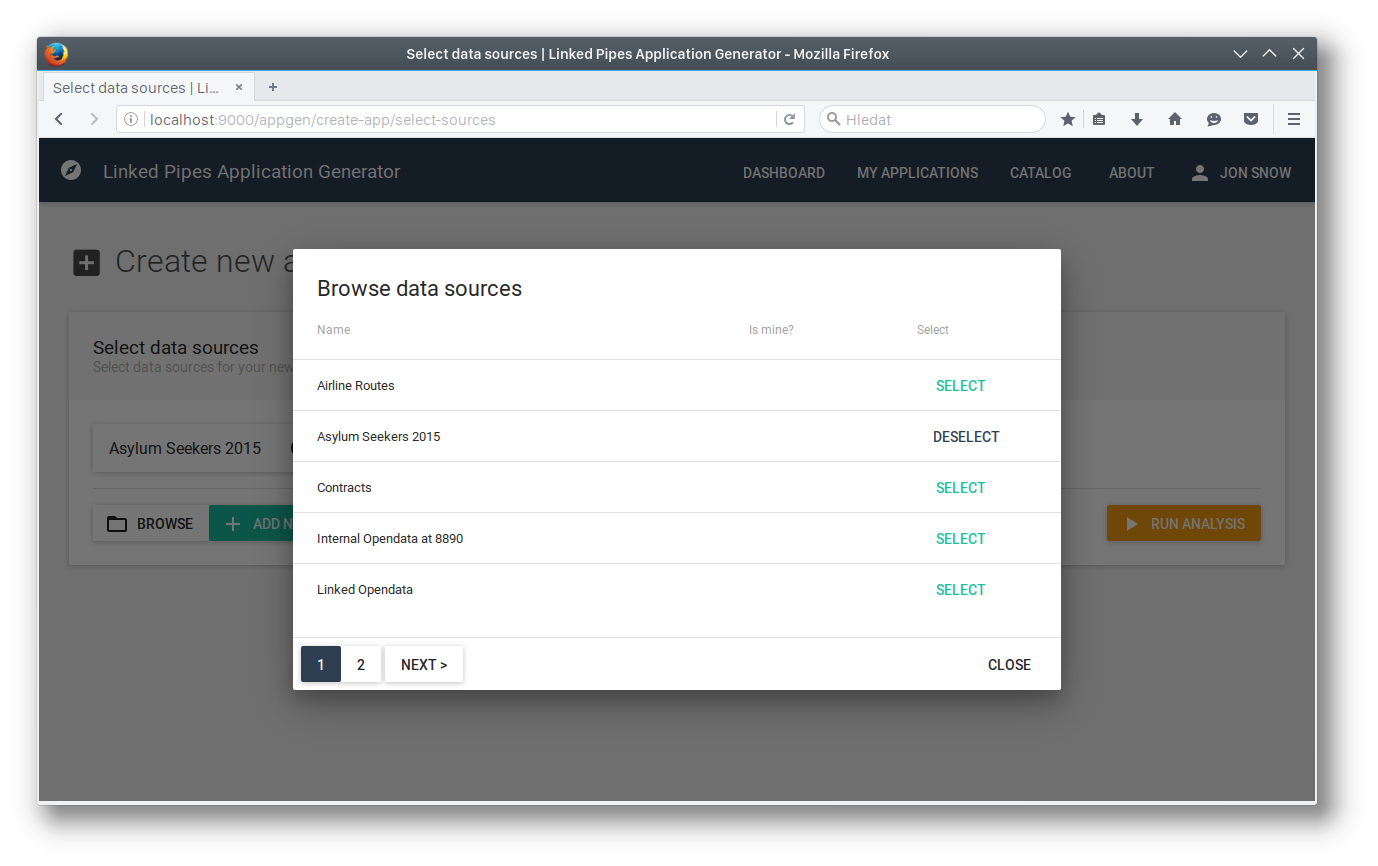
\includegraphics[width=145mm]{img/05_scenario_01_browse_data_sources.png}
	\caption{Asylum Seekers scenario: Browser locally available data sets. The journalist selects the Asylum Seekers 2015 data set.}
	\label{fig:scenario-01-browse-data-sources}
\end{figure}
\begin{figure}
	\centering
	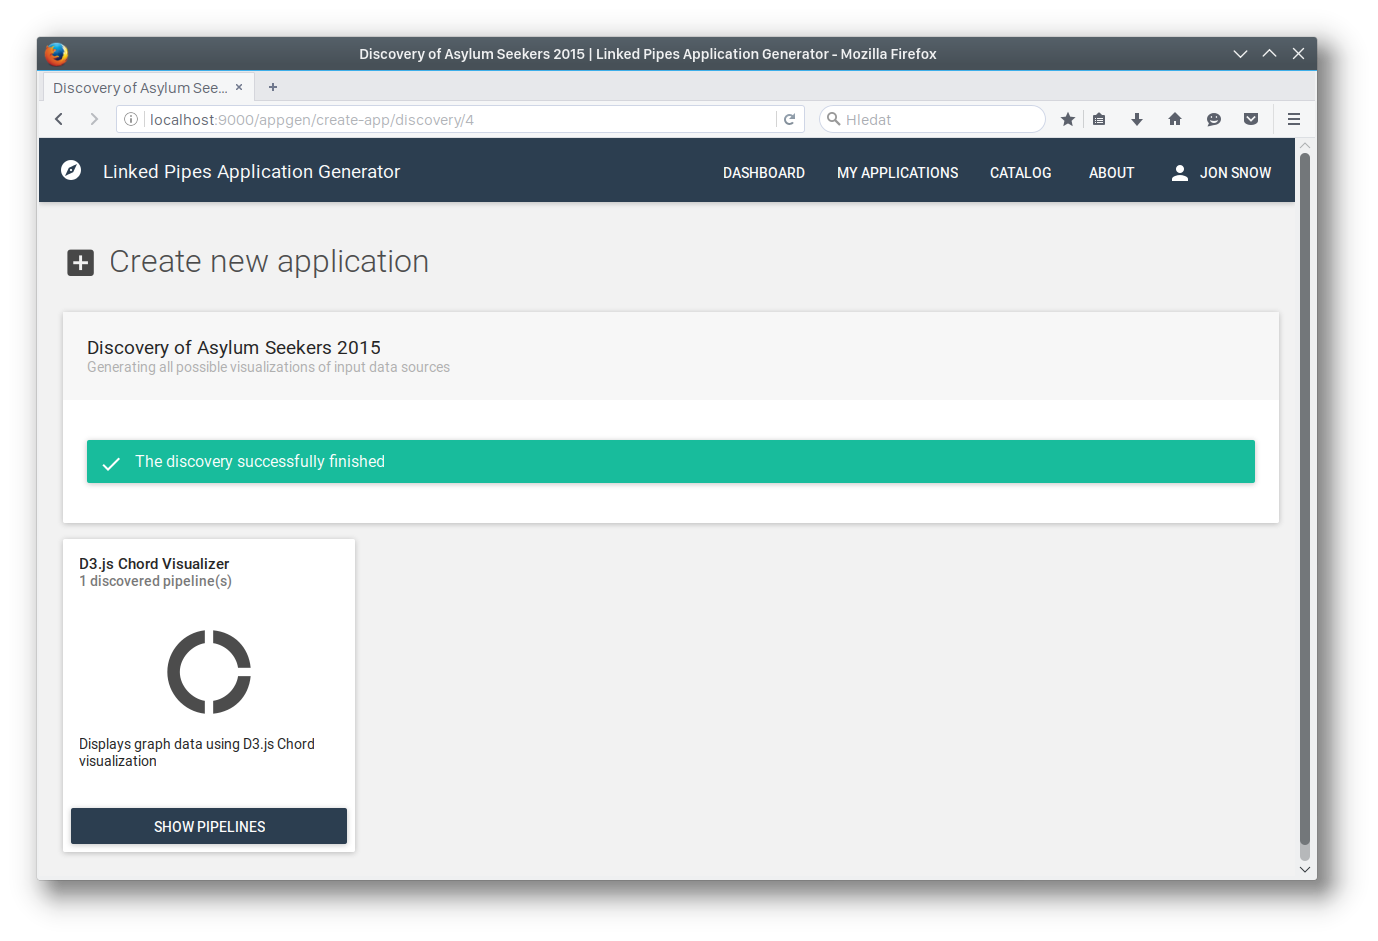
\includegraphics[width=145mm]{img/05_scenario_02_discovery_result.png}
	\caption{Asylum Seekers scenario: Discovery result. The journalist can see that the Asylum Seekers 2015 data set can be visualized only using the D3.js Chord Visualizer. He runs the one discovered LDVM \emph{pipeline} that ends with this particular LDVM \emph{visualizer component}.}
	\label{fig:scenario-02-discovery-result}
\end{figure}
\begin{figure}
	\centering
	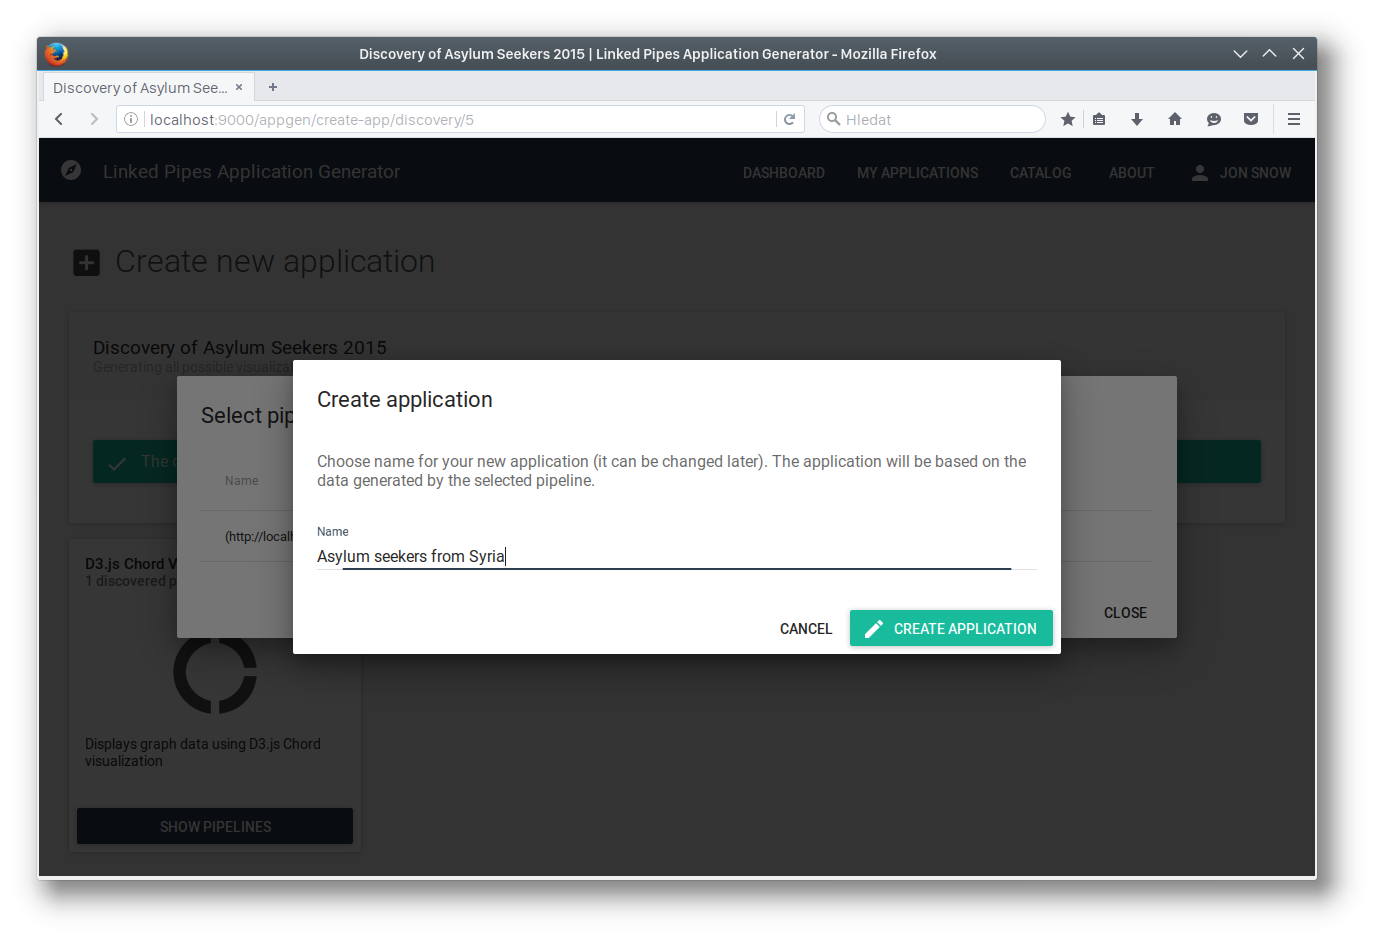
\includegraphics[width=145mm]{img/05_scenario_03_create_application.png}
	\caption{Asylum Seekers scenario: Create application dialog. When the \emph{pipeline evaluation} is done, the user can proceed by creating an application.}
	\label{fig:scenario-03-create-application}
\end{figure}

\begin{figure}
	\centering
	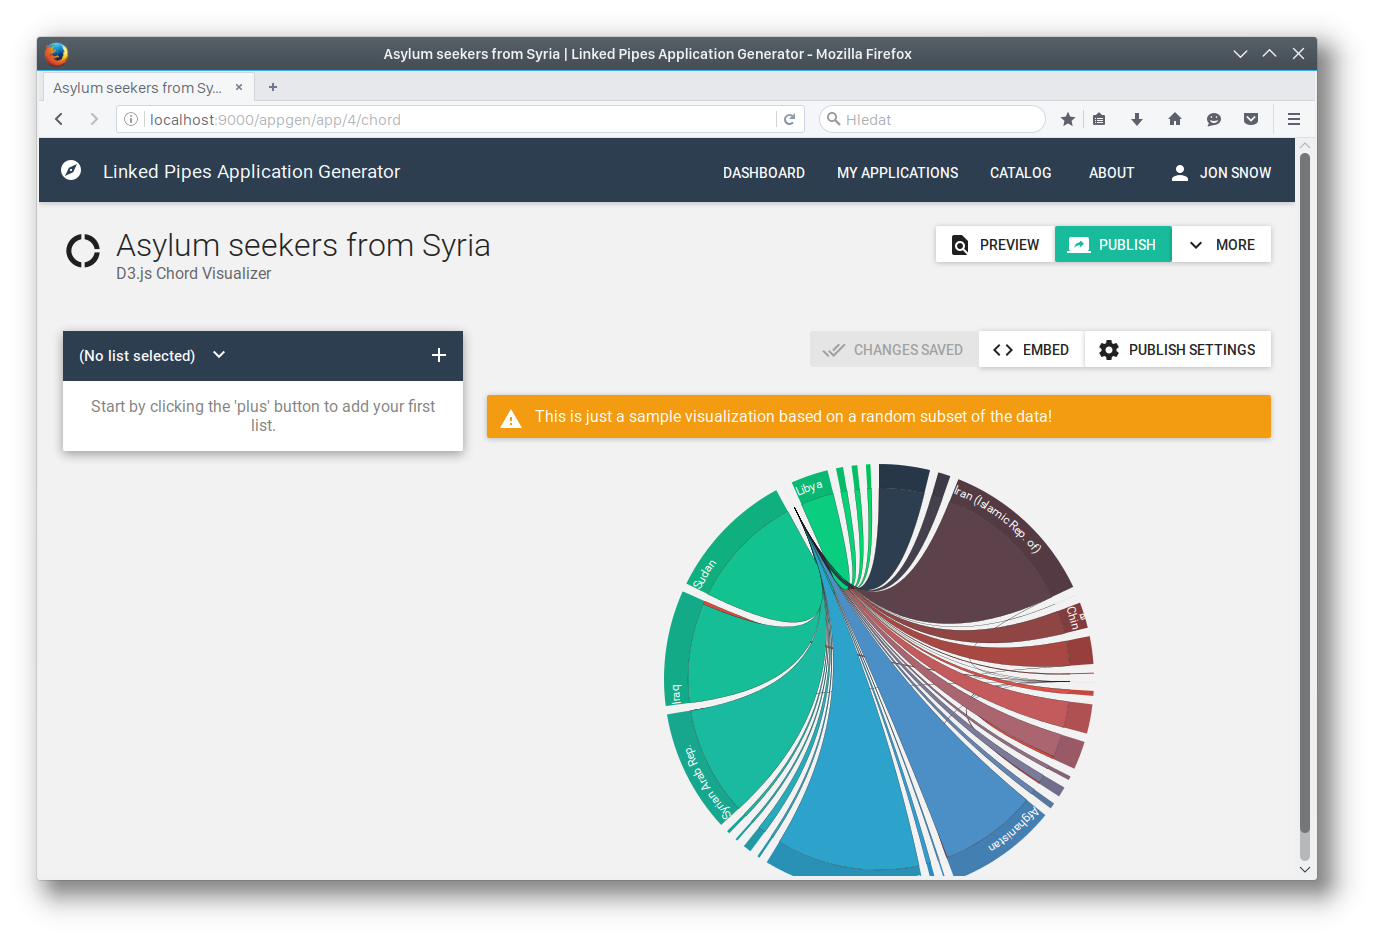
\includegraphics[width=145mm]{img/05_scenario_04_graph_sample.png}
	\caption{Asylum Seekers scenario: Configurator of D3.js Chord Visualizer. Immediately after the application is created, the journalist is presented with a random sample visualization of the data.}
	\label{fig:scenario-04-graph-sample}
\end{figure}
\begin{figure}
	\centering
	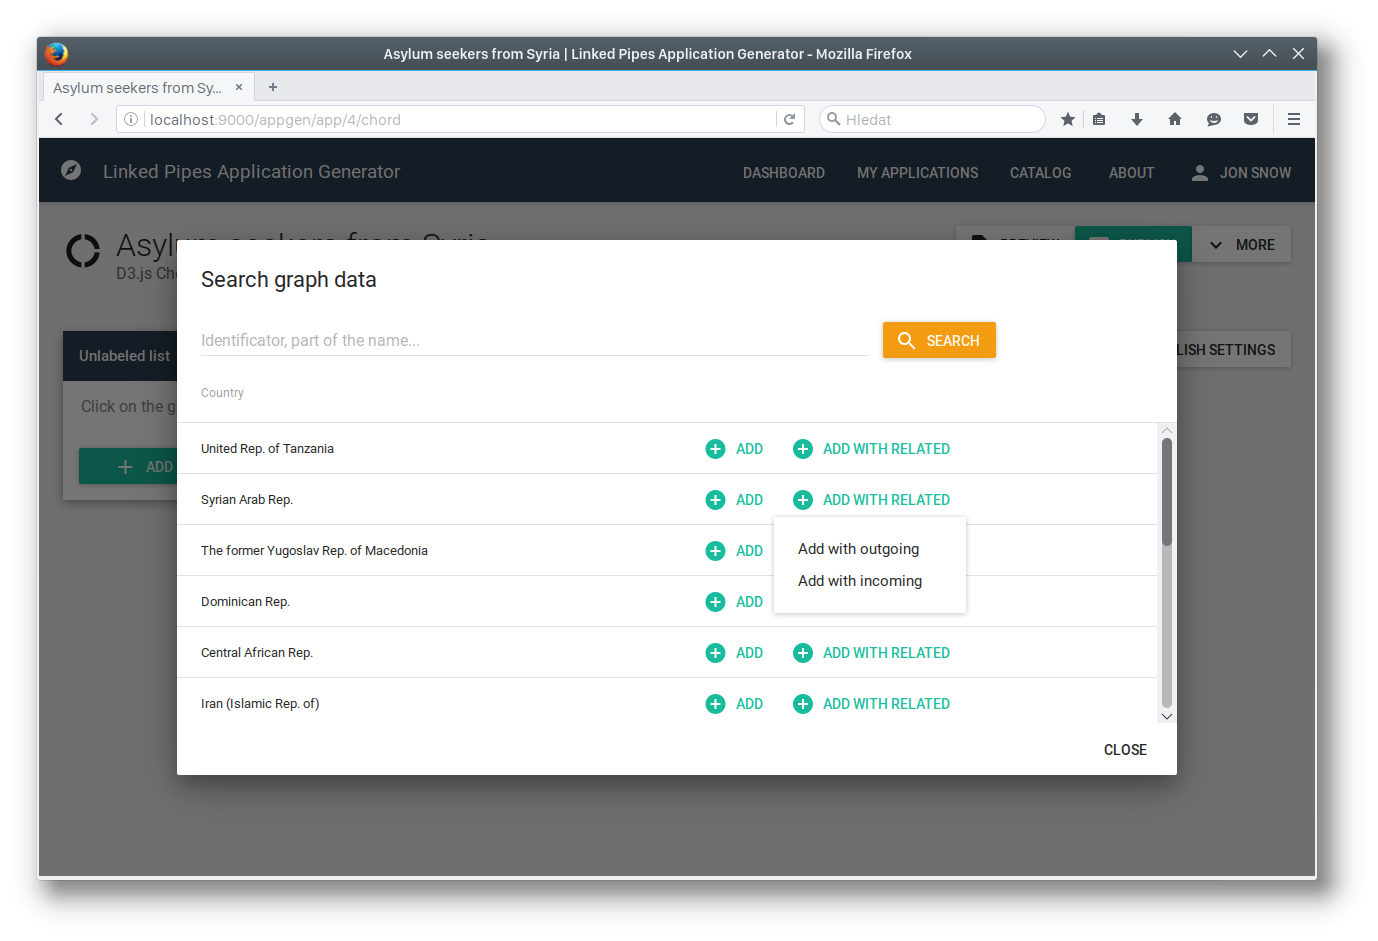
\includegraphics[width=145mm]{img/05_scenario_05_search_graph}
	\caption{Asylum Seekers scenario: Search dialog. The journalist wants to make a visualization of asylum seekers coming from Syria. He creates a new  \emph{list} (a \emph{list} contains entities that should be visualized using a single diagram). The journalist uses the search feature to find Syria in the data set and adds it together with all target countries to the new \emph{list}.}
	\label{fig:scenario-05-search-graph}
\end{figure}
\begin{figure}
	\centering
	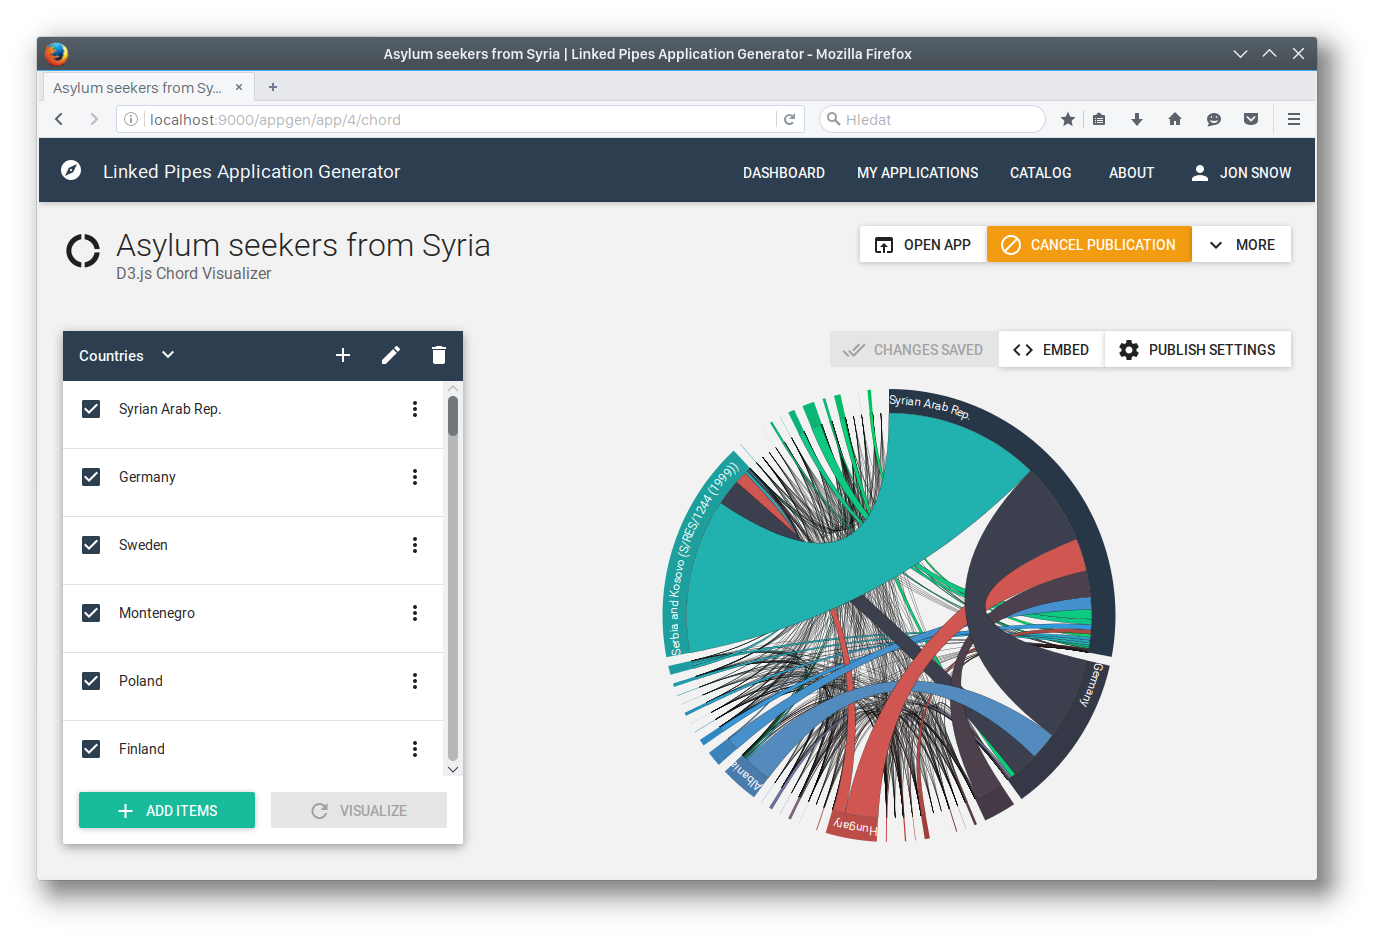
\includegraphics[width=145mm]{img/05_scenario_06_ready_application}
	\caption{Asylum Seekers scenario: Visualization of selected countries. The journalist is now presented with the chord diagram of the countries he added into the \emph{list}.}
	\label{fig:scenario-06-ready application}
\end{figure}
\begin{figure}
	\centering
	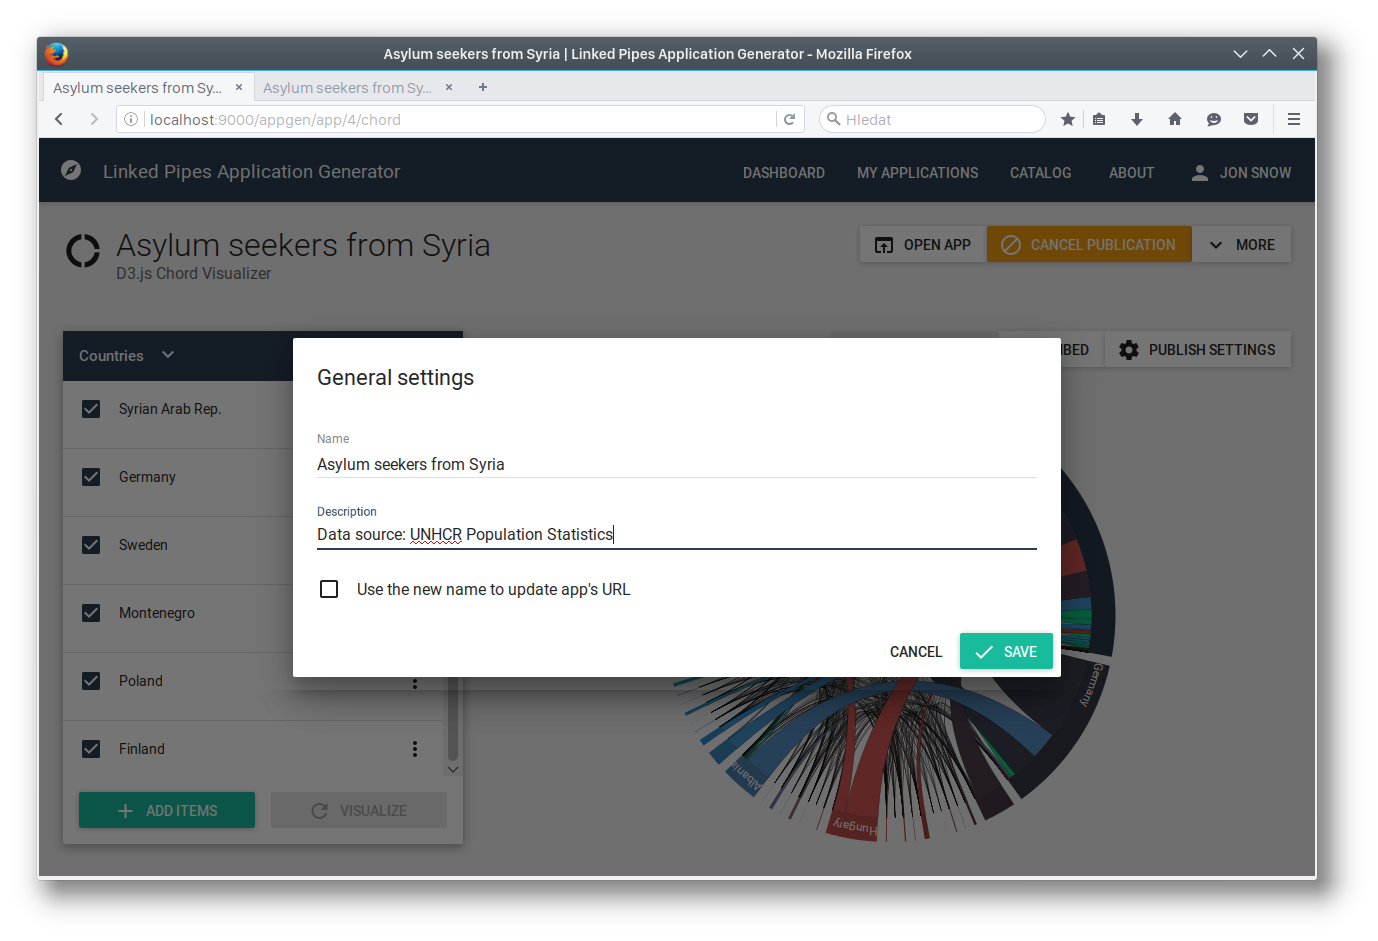
\includegraphics[width=145mm]{img/05_scenario_07_general_settings}
	\caption{Asylum Seekers scenario: General application settings. The journalist can also provide the application description (in this case he uses it to explicitly mention the source of the data).}
	\label{fig:scenario-07-general-settings}
\end{figure}
\begin{figure}
	\centering
	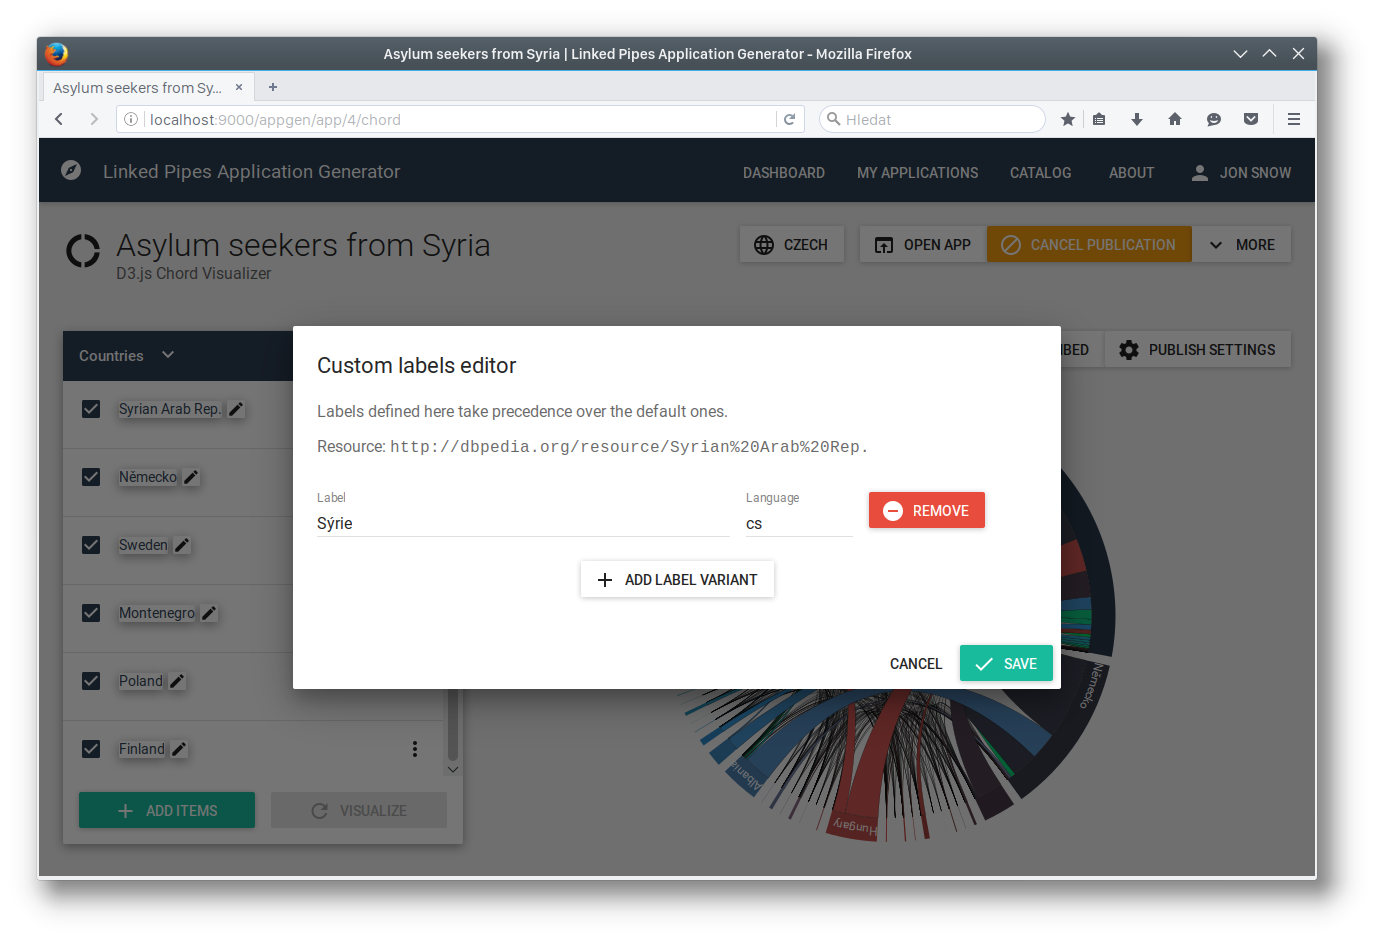
\includegraphics[width=145mm]{img/05_scenario_08_custom_label_editor}
	\caption{Asylum Seekers scenario: Custom labels editor. The journalist is targeting Czech audience but the country names in the data set are in English. The configurator lets the journalist provide his own names that will override the default ones. }
	\label{fig:scenario-08-custom-label-editor}
\end{figure}
\begin{figure}
	\centering
	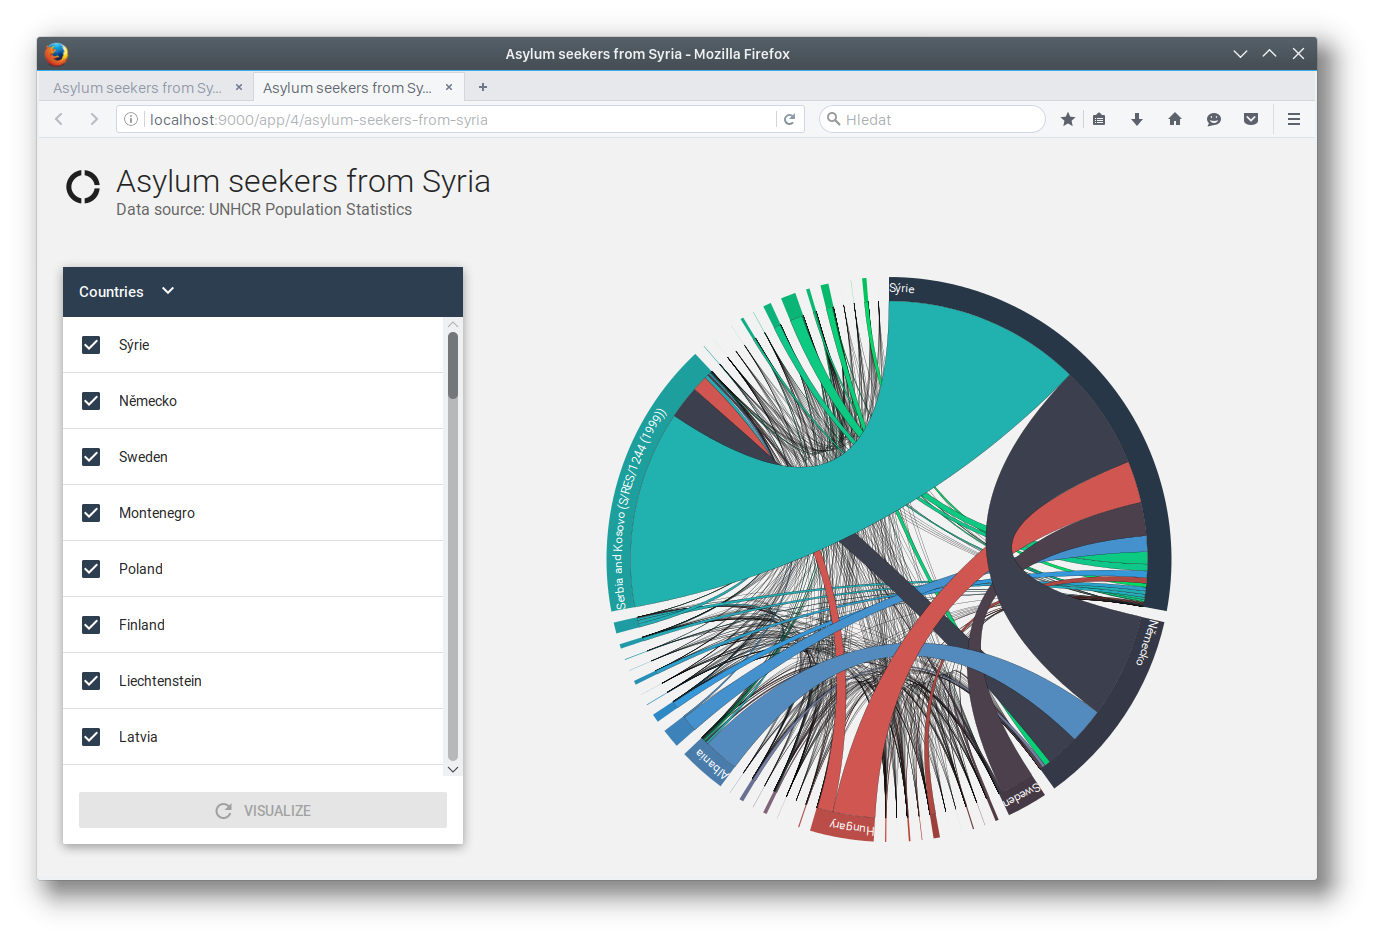
\includegraphics[width=145mm]{img/05_scenario_09_published_app}
	\caption{Asylum Seekers scenario: Published application. This is what the journalist's readers will see when the application gets published. Using the menu on the side, the users can switch on/off individual countries in the chord diagram.}
    \label{fig:scenario-09-published-app}
\end{figure}
\begin{figure}
	\centering
	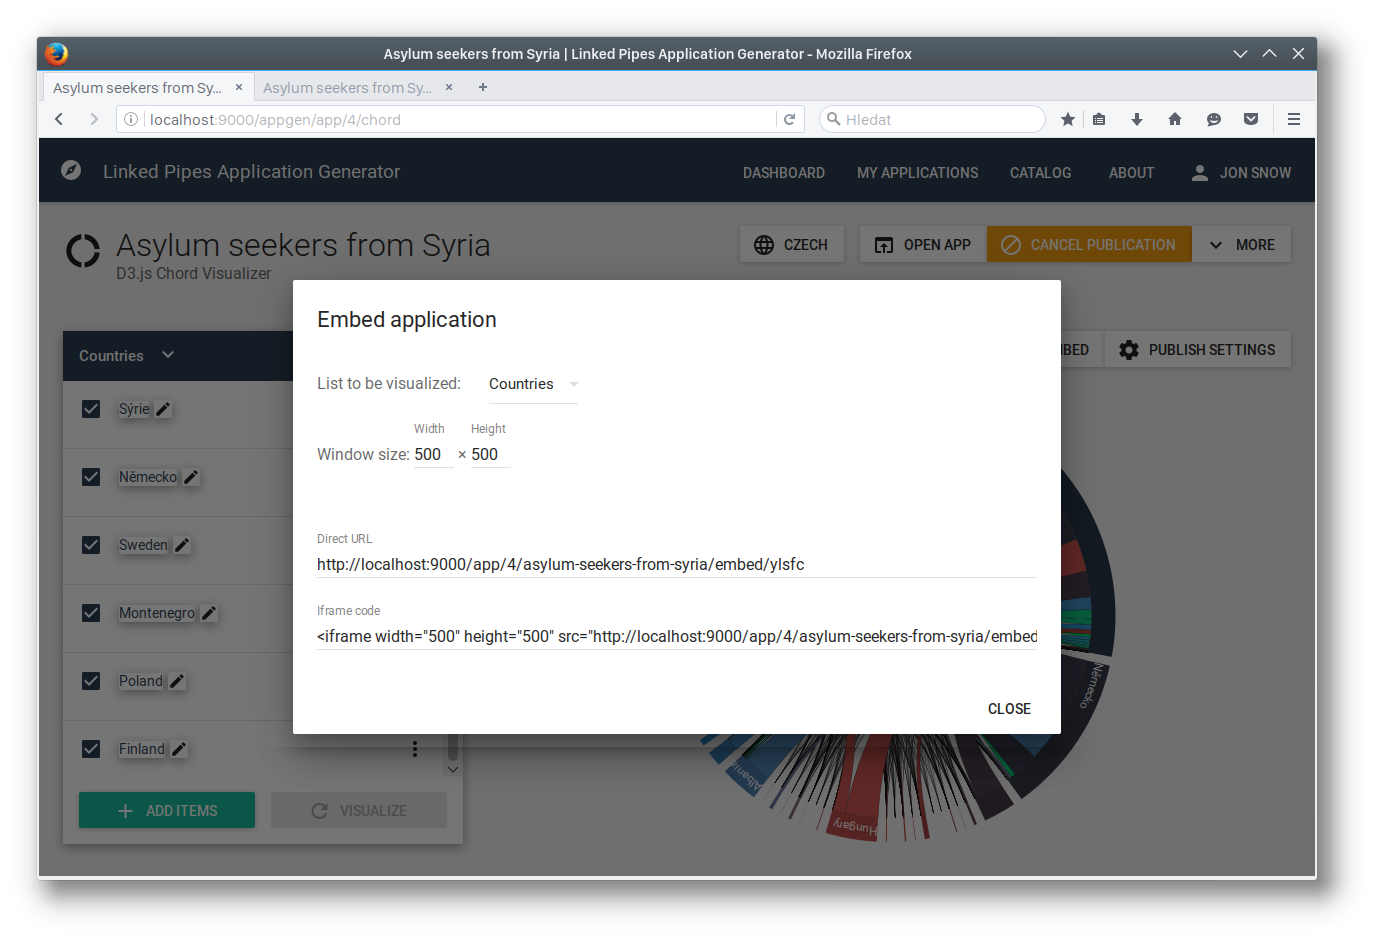
\includegraphics[width=145mm]{img/05_scenario_10_embed_application}
	\caption{Asylum Seekers scenario: Embed application dialog. The journalist may decide to embed the chord diagram directly into his article.}
    \label{fig:scenario-10-embed-application}
\end{figure}
\begin{figure}
	\centering
	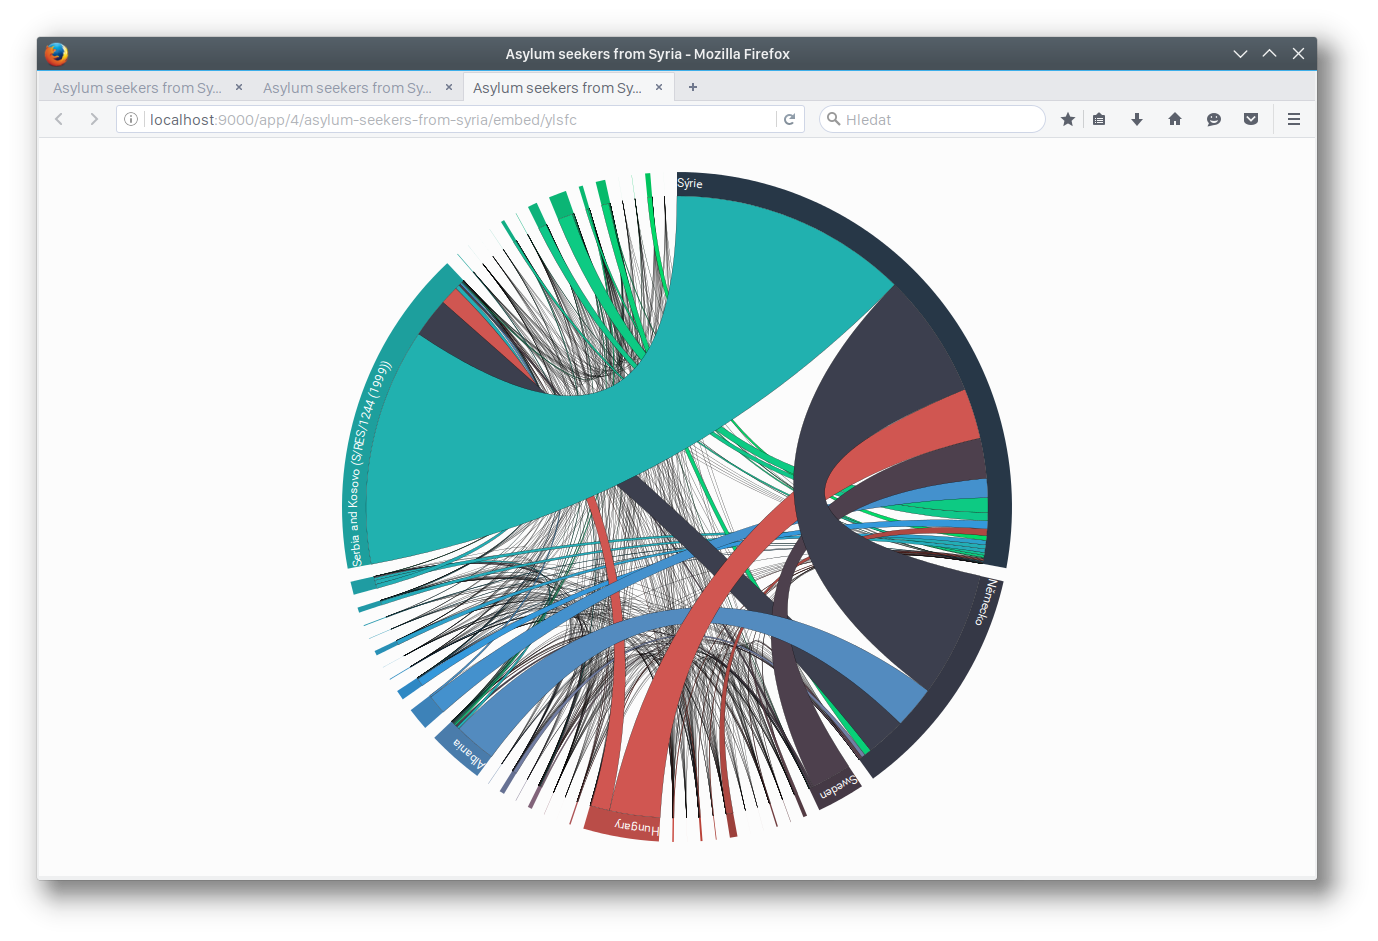
\includegraphics[width=145mm]{img/05_scenario_11_embedded_application}
	\caption{Asylum Seekers scenario: Embedded application. In this form, stripped from all controls to the bare visualization, it is perfect for direct embedding into web pages.}
    \label{fig:scenario-11-embedded-application}
\end{figure}


\subsection{Users}
\label{sec:implementation:overview:users}

Everyone who wants to use our \emph{application generator} needs to create an account first. At this moment, a user can either create a standard local account protected by a password or he can log in with his Google account (using OAuth 2.0 based Google Sign-In authentication system\footnote{\url{https://developers.google.com/identity/sign-in/web/}}). No other providers are currently supported. As the user works with the \emph{application generator}, all his applications, data sources and discoveries are linked to his account and no one else can access it. E.g. an application can be configured only by its owner and before it is published, only the owner can view it.

One exception are \emph{administrator} accounts which work similarly to root users known from Unix systems. Such users can access and update any applications, data sources or discoveries in the system. The first user to register in our \emph{application generator} automatically becomes an administrator. The others have to be manually appointed (which is currently not possible through the user interface and has to be done by directly updating the database record).

\begin{figure}
	\centering
	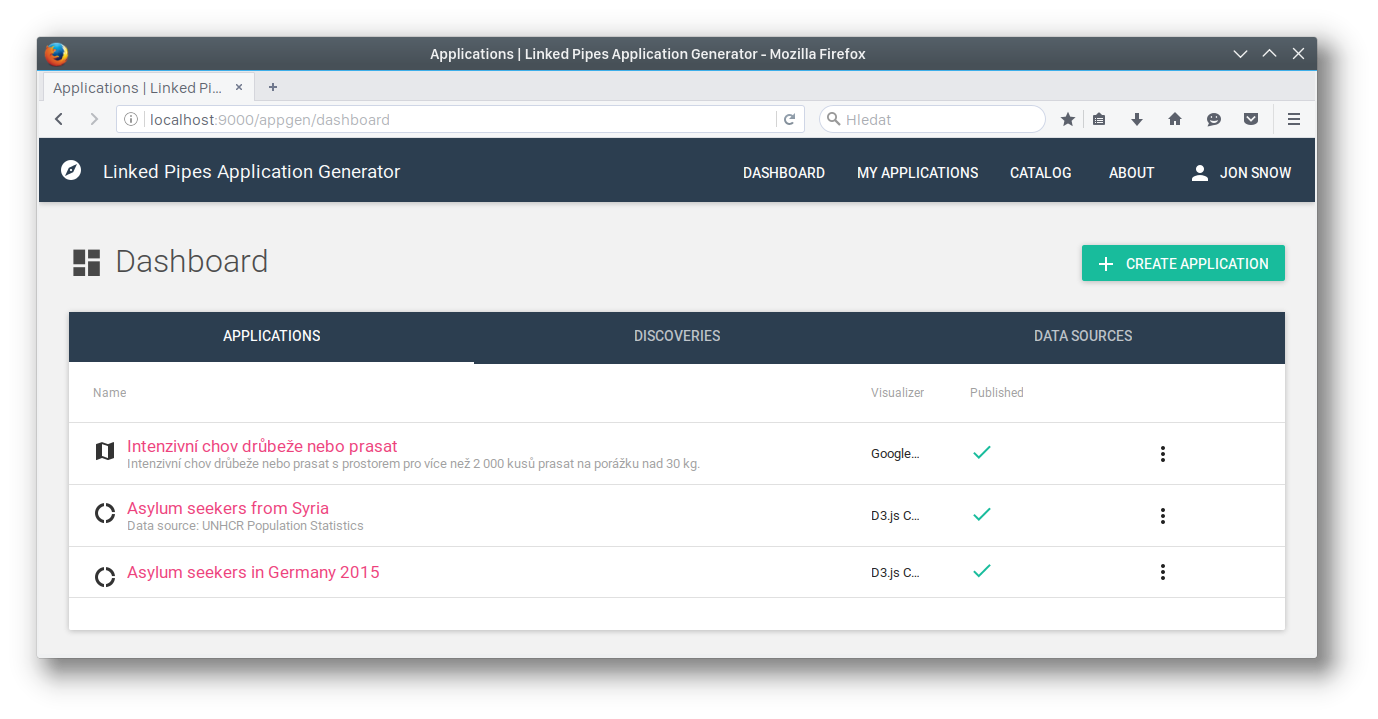
\includegraphics[width=145mm]{img/05_dashboard}
	\caption{User dashboard showing the overview of applications, discoveries and data sources}
    \label{fig:dashboard}
\end{figure}

\subsection{Data sources}

Our  approach to data sources is slightly different to LinkedPipes Visualization. In LinkedPipes Visualization, the user starts by providing the data source (may it be the SPARQL endpoint URL or a *.ttl file with serialized RDF data) and he has to do it every single time he wants to create a visualization. In our \emph{application generator}, we focused more on the possibility to re-use and share the data sets. So the user has to start by adding a data source to the generator, giving it a common name and only then he is allowed to select it for visualization. This data source remains linked to his account (i.e., he is the owner of this data source) which is also a significant change compared to LinkedPipes Visualization.

We distinguish between public and private data sources. Private data sources are seen only by their owner (it should be mentioned that they are just hidden by the user interface, they are not actively protected from being used by other users). Public data sources, on the other hand, ale openly available for anyone and can be selected in the data source browser (Figure \ref{fig:scenario-01-browse-data-sources}). Any user can decide to make any of his data sources public (when he is adding the data source or any time later). The idea is that one user (a data expert) might prepare the data set and another might use it to generate an application.

This approach introduces another level of abstraction. The user generating an application does not have to know what RDF or a SPARQL endpoint is, i.e, he is separated from the technical details. He can simply browse the publicly available data sources and select those that he is interested in.

\subsection{Pipeline discovery}

The \emph{application generator} runs the underlying LDVM \emph{discovery} algorithm on the selected data sources. The \emph{discovery} returns all possible LDVM \emph{pipelines} that lead to a visualization, i.e., they end with a \emph{visualizer component}. Multiple \emph{pipelines} might use the same \emph{visualizer component} (they might use different \emph{analyzers} and \emph{visualizer transformers} along the way to get the input data compatible with this particular visualizer).

Unfortunately, we are not able to give the user any detailed information about how the data produced by a \emph{pipeline} will look like. The reason is that the \emph{pipelines} are assembled using a static \emph{compatibility} check as explained in Section~ \ref{sec:linkedpipes:ldvm-implementation}. The compatibility check guarantees that the \emph{pipeline} will produce some data that are visualizable by the \emph{visualizer} but it cannot provide any more information about the actual data quality. The only way to find out is to actually execute the \emph{pipeline} and create an application from it. If the data do not make sense or are not what the user expects, the user can try another one.

The user can watch the \emph{discovery} algorithm progress on a dedicated screen that shows the current \emph{discovery} status and also the list of \emph{pipelines} that have been discovered so far (Figure \ref{fig:scenario-02-discovery-result}). The \emph{pipelines} are grouped by \emph{visualizers}. As the algorithm may take some time, the user can leave the screen and come back later. It is accessible even after the \emph{discovery} algorithm finishes. The list of all discoveries can be found on the dashboard \ref{fig:dashboard}.

Note that not all \emph{visualizers} are supported by our \emph{application generator} (i.e., the corresponding \emph{plugin} is missing). For example, LinkedPipes Visualization contains a \emph{visualizer} for statistical data described using Data Cube Vocabulary \cite{datacube_vocabulary}. If the appropriate LDVM \emph{component} is registered in our \emph{application generator}, the \emph{discovery} algorithm will return \emph{pipelines} that use this \emph{component}. However, those will not be offered to the user (the \emph{application generator} will inform the user that this particular \emph{visualizer} is not supported).

\subsection{Application configuration}

The configuration phase is the core feature of the \emph{application generator} which differentiates it from the LinkedPipes Visualization. The application configuration involves both tasks that are common for all applications (e.g. publishing, deleting, updating description etc.) and that are \emph{visualizer} specific. As you can see on the Figure \ref{fig:configurator}, the \emph{configurator} interface follows this principle. It is divided into the common area and the area which is controlled by a particular \emph{visualizer} plugin (see Figure \ref{fig:google_maps_visualizer} of how a different \emph{visualizer} adapts to the universal configurator interface). 

\begin{figure}
	\centering
	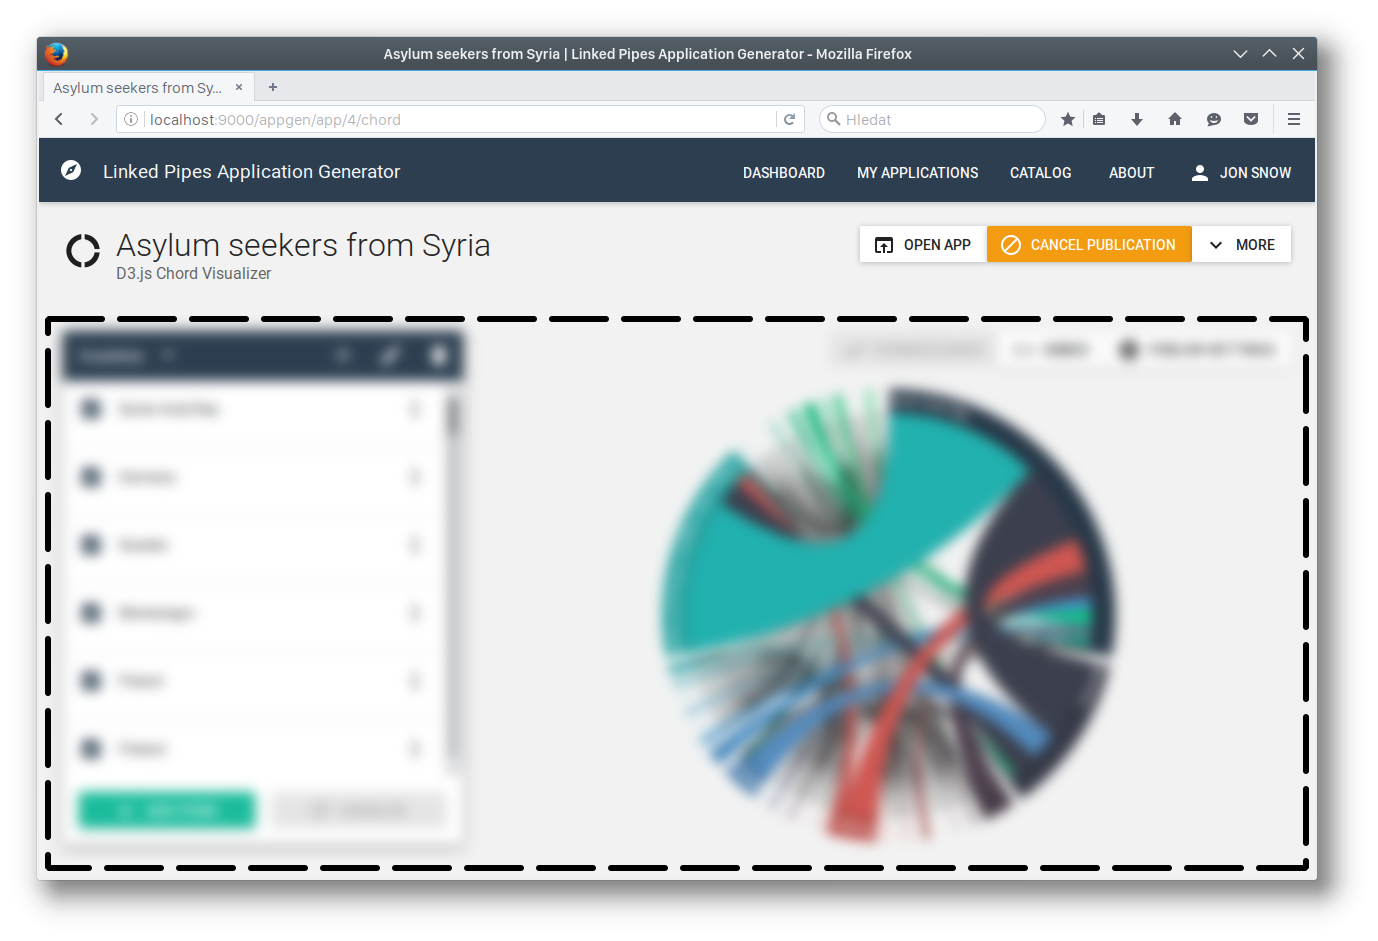
\includegraphics[width=145mm]{img/05_configurator.png}
	\caption{The configurator interface. The blurred out part with the dashed border is controlled by the current visualizer whereas the rest is identical for all visualizers. It contains the common functionality (e.g. the "More" button in the upper right corner shows a menu allowing the user to delete the application or change the application name and description).}
    \label{fig:configurator}
\end{figure}

\begin{figure}
	\centering
	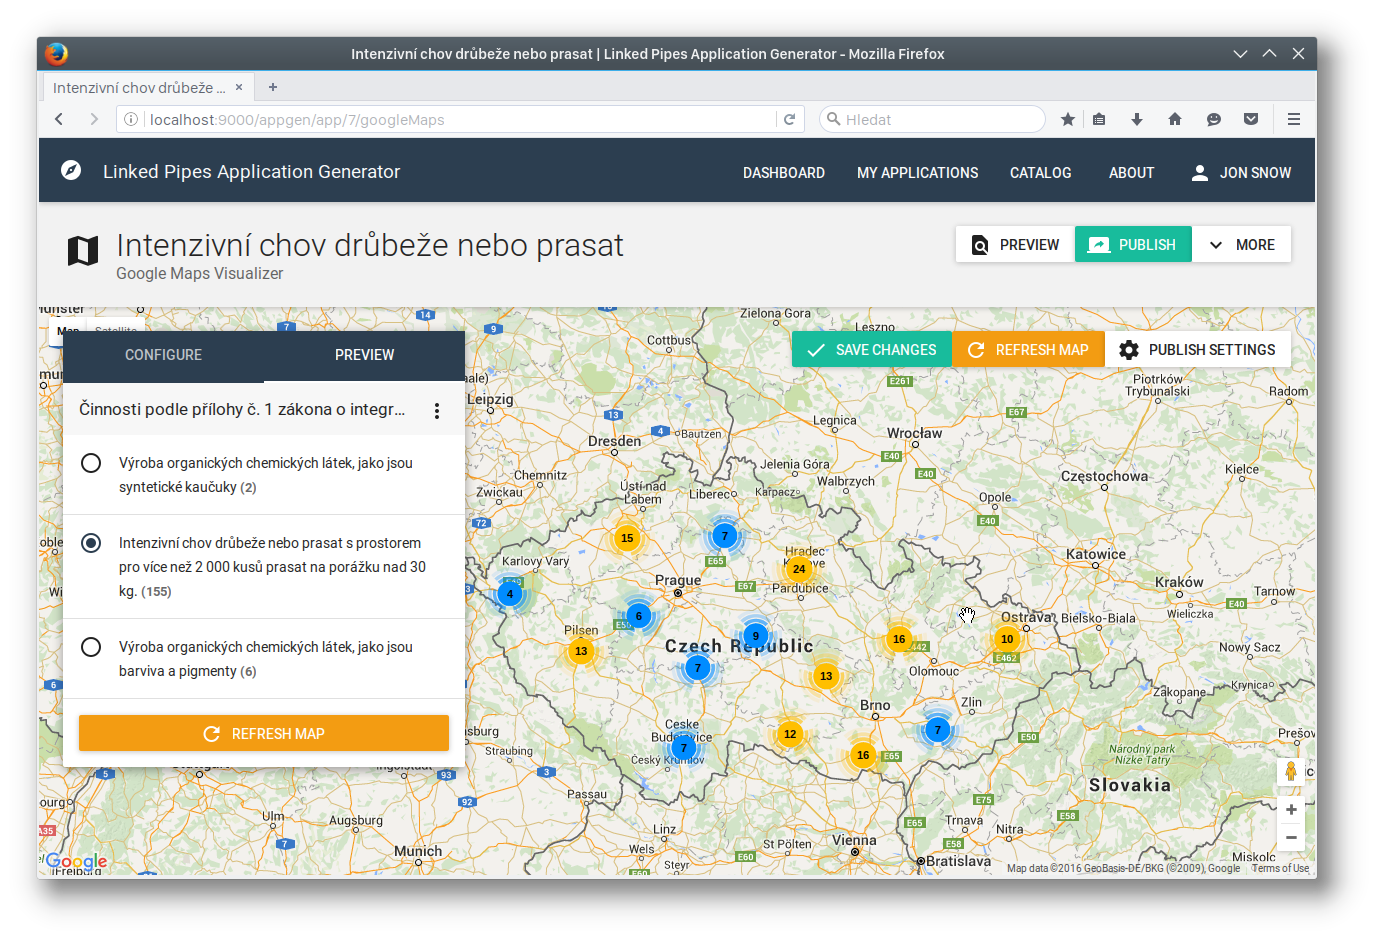
\includegraphics[width=145mm]{img/05_google_maps_visualizer.png}
	\caption{The configurator interface of the Google Maps Visualizer.}
    \label{fig:google_maps_visualizer}
\end{figure}

\subsection{Publishing applications}

When the user is happy with how the configuration looks, he can publish it by hitting the green "Publish button" (as seen for example on the Figure \ref{fig:scenario-04-graph-sample} in the upper right corner). The application then becomes accessible on a public URL which is generated from the application ID (internal numeric identificator) and its name. The \emph{application generator} at this moment does not offer any fine grained control of who gets to access the application. It is either public or not. Once published, it also becomes a part of the public application catalog (Figure \ref{fig:catalog}).

\begin{figure}
	\centering
	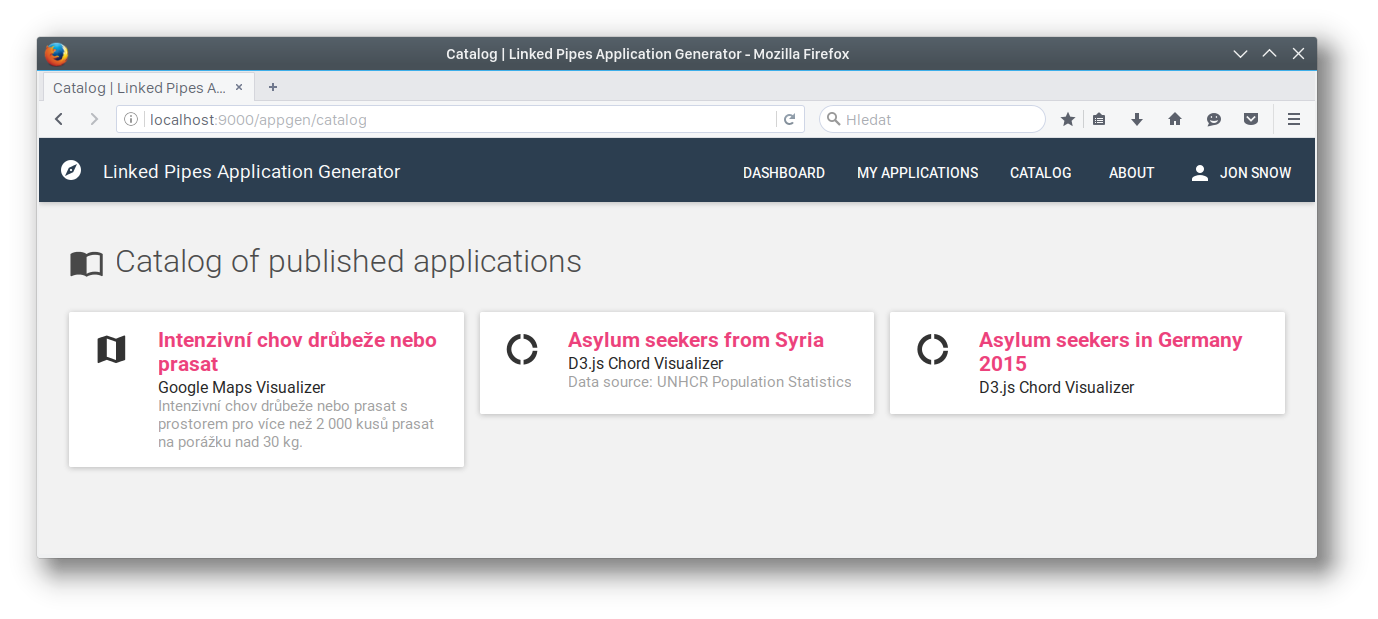
\includegraphics[width=145mm]{img/05_catalog}
	\caption{Catalog of published applications.}
    \label{fig:catalog}
\end{figure}

Some \emph{visualizers} offer the option to publish the application in an embed mode. That means that the application's interface is adapted so that it can be inserted for example into an external online article. The interface is usually significantly reduced and stripped from unimportant  control elements. This functionality is not considered common for all \emph{visualizers}  as each \emph{visualizer} can approach it differently. For example, the D3.js Chord Visualizer we used in this section allows the user to create multiple chord diagrams within a single application. Each of these diagrams can be exported separately in the embed mode (a unique URL is generated for each diagram under which the diagram is accessible). See Figure \ref{fig:scenario-10-embed-application}. Clearly, this functionality is specific for D3.js Chord Visualizer.

\section{Backend implementation}

Implementation-wise, the backend is fairly simple compared to the frontend. Everything important has been already covered in the corresponding analytical part of this text (Section~\ref{sec:system-proposal:architecture-analysis:backend}). The backend of LinkedPipes Visualization is powered by Play Framework\footnote{\url{https://www.playframework.com/}} which follows the MVC architecture and is written in Scala. As explained, we simply extend the existing backend codebase with controllers and services (or repositories) that cover the functionality of the \emph{application generator}. 

One of our concerns was to keep the \emph{application generator} as separated as possible from the original codebase. Therefore all our controllers are in a separate Scala package \texttt{controllers.appgen} and similarly all our services and repositories can be found in a separate Scala package \texttt{model.appgen}. The only exception are the services that we developed to add support for new RDF vocabularies. We do not consider these services to be the \emph{application generator} exclusive as they can be utilized by the LinkedPipes Visualization as well. Therefore when implementing them, we followed the structuring suggested by the authors of LinkedPipes Visualization.

\section{Frontend development stack}
\label{sec:implementation:frontend-development-stack}

As we explained in Section~\ref{sec:system-proposal:architecture-analysis:frontend-integration}, the \emph{application generator} frontend is completely separated from the LinkedPipes Visualization frontend. It uses a different development stack (set of tools) which is rather new and very specific. It includes React~\cite{react}, Redux~\cite{redux}, Reselect~\cite{reselect} and React-router~\cite{react-router}. 

In Section~\ref{sec:system-proposal:architecture-analysis:frontend-architecture} we covered the conceptual architecture of the frontend so the reader should have a general idea of how it works. However, in order for us to be able to convince the reader that our \emph{application generator} can work as a \emph{framework} for developing new \emph{visualizers}, we need the reader to understand the \emph{application generator} on a code level. Therefore we attached to this thesis a brief introduction (Attachment ~\ref{att:devstack}) that should get the reader familiar enough with these tools so that he can understand the following sections. Anyone who feels already familiar with these tools, can skip this part.

We should mention that Attachment~\ref{att:devstack} describes essentially the same ideas as Section~\ref{sec:system-proposal:architecture-analysis:frontend-architecture}, but on implementation level. 

\section{Frontend framework conventions}
\label{sec:implementation:frontend-conventions}

The tools that we have chosen for our frontend (Section \ref{sec:implementation:frontend-development-stack}) define the overall frontend architecture and the internal mechanisms (Section~\ref{sec:system-proposal:architecture-analysis:frontend-architecture}). Clearly, there is no monolithic framework. Each tool solves only one problem and even though they have been all designed to work well together and complement each other, there is missing an overall architecture and design patterns for large scale applications (something that a monolithic framework, such as Play Framework that we use in backend, usually offers).

There exist recommendations and patterns but they evolve just as quickly and erratically as the modern world of JavaScript frontend itself. While developing the \emph{application generator} (and turning into a \emph{framework}) we had to choose the right patterns and conventions for us and sometimes even come up with some new patterns.

This involves literary everything from the very basic questions of how our code should be organized to which library should we use to generate forms or how we should implement visual feedback for asynchronous requests. In this section we will focus mainly on the basic aspects which involve the code organization which is important because it affects the process of integrating new \emph{visualizers}.

Note that these conventions and patterns present a significant contribution from our side. Whereas the core architecture concepts, as described in Section~\ref{sec:system-proposal:architecture-analysis:frontend-architecture}, were to a large extent just given to us through the chosen development stack, it is these conventions and patterns that adopt the concepts, taking them from simple demos to a rather large, complex and extendable application as our \emph{application generator} is.

\subsection{JavaScript bundles}

As explained, our frontend code is written in ES6 and has to be compiled (or more correctly \emph{transpiled}) into standard JavaScript that any browser can understand. The frontend codebase consists of large amount of (not only) ES6 files which are all transpiled and put together into a single JavaScript file which we call a \emph{bundle}. This bundle is loaded to the web browser and contains everything that is required to run the SPA. We use Webpack bundler \footnote{http://webpack.github.io/} to put our code together and Babel \footnote{http://babeljs.io/} transpiler to convert our code.

The disadvantage of this approach is that this bundle is typically relatively large (3-4 Megabytes at this moment) and therefore takes some time to load. Before it loads, the user does not see anything on the screen. On the other hand, once it is loaded, the user experience is very smooth because we do not have to make any more request to the server to fetch additional resources.

Our \emph{application generator} consists of several bundles which correspond to the different SPAs (Figure~\ref{fig:frontend-base-structure-spas}). The main is the \emph{platform} bundle which contains the whole \emph{platform} user interface and also \emph{configurator} interfaces for all registered \emph{visualizers}. Then every registered \emph{visualizer} has its own bundle that contains only the \emph{application} interface. This bundle is used for published applications and as it does not contain the whole platform, it is significantly smaller and faster to load.

Even though we have multiple bundles, all the code exists in one spot. The reason is that there is very little code that is used only in a single bundle and therefore it would not make sense to separate it in any way. What defines a bundle is an \emph{entry point} which is a simple JavaScript file where Webpack starts the bundling process.

\subsection{Code structure}

The frontend code is all in the folder \texttt{src/app/assets\_webpack/appgen}. We will refer to this folder as to the \texttt{assets} folder. There are two subfolders \texttt{javascripts} and \texttt{stylesheets} with self-explanatory names. What is interesting is that the styles are also included into the bundle.  Let us now quickly walk through the folders in \texttt{javascripts}.

\begin{itemize}
\item \textbf{components} -- useful single-purpose React components
\item \textbf{containers} -- the top level React components that are connected to Redux
\item \textbf{entries} -- Webpack entry points (each file here corresponds to a bundle)
\item \textbf{misc} -- various utilities
\item \textbf{modules} -- the actual code
\item \textbf{store} -- instantiation of Redux \emph{store}

\end{itemize}
\subsection{Ducks}

Our code contains lots of Redux \emph{actions}, \emph{reducers} and Reselect \emph{selectors}. A common pattern is to put all \emph{actions} into the \texttt{actions.js} file, all \emph{reducers} into the \texttt{reducers.js} file and all selectors into a \texttt{selectors.js} file. In our \emph{application generator}, we decided to adopt the \emph{duck} format \footnote{https://github.com/erikras/ducks-modular-redux}. The idea is that we put all \emph{actions}, \emph{reducers} and \emph{selectors} related to the same functionality into a single file called a \emph{duck}. 

We take the example from Section \ref{att:devstack:redux} where we were explaining how Redux works and rewrite it into the duck format. This would be a single file (i.e., an ES6 module).

\begin{verbatim}
// Actions 

export const INCREMENT = ’INCREMENT’;
export function increment() {
  return { type: INCREMENT };
}

export const DECREMENT = ’DECREMENT’;
export function decrement() {
  return { type: DECREMENT };
}

// Reducer

export default function valueReducer(state = 0, action) {
  switch (action.type) {
    case INCREMENT:
      return state + 1
    case DECREMENT:
      return state - 1
    default:
      return state
    }
}

// Selectors

export const valueSelector = state => state.value;
\end{verbatim}

This \emph{duck} covers the complete functionality regarding incrementing and decrementing a value. It exports public API for updating the value (\emph{action creators}), reading the value (\emph{selectors}) and it defines how the value should be represented and updated (\emph{reducer}). The \emph{action types} are exported as well which means that anyone can listen to these \emph{dispatched} \emph{actions}. In \emph{object-oriented programming} terminology we could say that the \emph{action creators} correspond to object \emph{setters} and \emph{selectors} to object \emph{getters} (note that we already mentioned \emph{ducks} in Section~\ref{sec:system-proposal:architecture-analysis:frontend-architecture} while describing the general frontend architecture).

\subsection{Modules}

Clearly, having all React components and all \emph{ducks} in a single place is not viable for large applications. Therefore we introduce a \emph{module} which is the base organization unit in our code (please do not confuse it with ES6 modules). A \emph{module} is similar to a \emph{package} from Java. It usually covers one area of functionality. For example, we have an \texttt{auth} \emph{module} that covers everything related to authenticating and registering users. Also every registered \emph{visualizer} has its own \emph{module}.

A \emph{module} is in the first place a folder with standardized content. Let us walk through folders that a \emph{module} typically contains.

\begin{itemize}
\item \textbf{components} -- React components that focus mainly on the visuals (\emph{view} components)
\item \textbf{containers} -- React components that are connected to Redux and handle business logic (\emph{controller} components)
\item \textbf{dialogs} -- React components for dialog windows
\item \textbf{ducks} -- \emph{ducks} required in this module
\item \textbf{misc} -- various utilities
\item \textbf{pages} -- React components that are bound to React-router routes
\end{itemize}

As a module covers a concrete functionality, it is very likely to define its own \emph{actions}. All \emph{action types} in one \emph{module} should have a common prefix corresponding to the \emph{module} name. Firstly, when an \emph{action} is dispatched, we can easily identify which \emph{module} it came from. Secondly, we do not have to worry about conflicting \emph{action types} (with the prefix we are creating a separated namespace). Therefore each \emph{module} needs to contain a \texttt{prefix.js} file.

\begin{verbatim}
// prefix.js

import createPrefixer from '../../../misc/createPrefixer'

export const MODULE_PREFIX = 'example';
export default createPrefixer(MODULE_PREFIX);
\end{verbatim}

The \texttt{MODULE\_PREFIX} should contain the \emph{module} name, i.e., the folder name containing the \emph{module}. We tried to come up with a solution which would automatically populate this constant with the folder name but that is, to our best knowledge, not possible due to how Webpack bundling process works. 

This is how we would use it in our \emph{duck} (following the \emph{module} structure, the \emph{duck} should be placed in \texttt{ducks/value.js}).

\begin{verbatim}
// ducks/value.js

import prefix from '../prefix.js'

// Actions 

export const INCREMENT = prefix(’INCREMENT’);
export function increment() {
  return { type: INCREMENT };
}

export const DECREMENT = prefix(’DECREMENT’);
export function decrement() {
  return { type: DECREMENT };
}
\end{verbatim}

The \emph{action types} are now \texttt{example/INCREMENT} or \texttt{example/DECREMENT}.

The \emph{modules} are meant to be nested, on the file system level (nesting folders) but also on the \emph{state} level.  Each \emph{module} has to define a root \emph{reducer} combining all its nested \emph{reducers}.

\begin{verbatim}
// reducer.js

import { combineReducers } from 'redux'
import value from './ducks/value' // the default export points to the reducer

const rootReducer = combineReducers({
  value
});

export default rootReducer;
\end{verbatim}

This root \emph{reducer} has to be added to the root \emph{reducer} of the parent \emph{module} in a similar manner. 

Complementary to \emph{reducers} are \emph{selectors}. Each \emph{module} defines its root \emph{selector}.

\begin{verbatim}
// selector.js

import { createSelector } from 'reselect'
import parentSelector from '../selector'
import { MODULE_PREFIX } from './prefix'

export const moduleSelector = createSelector(
  [parentSelector],
  parentState => parentState[MODULE_PREFIX]
);
export default moduleSelector;
\end{verbatim}

Note that the logic is inverted to how the \emph{reducers} are composed. Here we use the parent \emph{selector} to access the \emph{state} of the parent \emph{module} and we select the piece that belongs to our \emph{module}. This is given by the APIs of Redux and Reselect. We just have to make sure to use the same key when registering both the \emph{reducer} and the \emph{selector} (the \emph{module} name should be used as the key).

Using this approach, the \emph{state} hierarchy corresponds to the \emph{module} folder hierarchy. What is important is that this defines a clear way of how the application can be arbitrarily and endlessly extended with very little risk of conflicts. \emph{Modules} can be arbitrarily renamed and moved around. We just have to make sure to always connect the \emph{reducer} and the \emph{selector} to the right spot.

A \emph{module} can also contain routes that would be composable in a similar manner. The route structure, however, does not strictly follow the folder structure as the situation with routing is more complicated. For example, a \emph{module} representing a \emph{visualizer} defines two sets of routes: one for the \emph{configurator} interface and one for the \emph{application} interface.

\section{Framework usage: A guide to integrating new visualizers}
\label{sec:implementation:integrating-visualizer}

Now that the reader is equipped with all the necessary knowledge, we will walk him through the process of creating a brand new \emph{visualizer} to demonstrate the abilities of our framework. The \emph{visualizer} will be visualizing a graph (as understood in the graph theory) represented with the RGML vocabulary (which makes it very similar to the D3.js Chord Visualizer that will be properly described later, including the vocabulary). The purpose of this section is merely to get the reader familiar with the basic integration steps. The presented \emph{visualizer} will simply display number of vertices and edges of the graph and let the user configure the graph label.

Before we start, we would like to make one remark. We will walk the user through the whole process and along the way we will touch parts of the software that were not designed and developed by us but by the authors of LinkedPipes Visualization \cite{linked_pipes_visualization}. We do not want to take credit for those parts. Specifically, those are the parts shared with LinkedPipes Visualization, which means everything related to the LDVM implementation and low-level work with RDF data.

\subsection{Guide overview}

Let us start with a list of steps to give the reader an overview of what is ahead of us. The first five steps are mandatory in a way that they are necessary to get the \emph{visualizer} up and running. When the first five steps are done, it is possible to generate new applications with this new \emph{visualizer} (this among other things means that the \emph{discovery} is able to utilize the new \emph{visualizer} while looking for pipelines). The other four steps add some actual functionality to the \emph{visualizer}. This functionality includes extracting some RDF data from the \emph{pipeline output}, loading them to the frontend and showing them to the user.

\begin{enumerate}
\item LDVM \emph{component} (\ref{sec:implementation:integrating-visualizer:ldvm})
\item Frontend \emph{visualizer} module (\ref{sec:implementation:integrating-visualizer:2})
\item \emph{Configurator} user interface (\ref{sec:implementation:integrating-visualizer:configurator})
\item \emph{Application} user interface (\ref{sec:implementation:integrating-visualizer:4})
\item Linking LDVM \emph{component} to the \emph{plugin} (\ref{sec:implementation:integrating-visualizer:5})
\item Scala backend  (\ref{sec:implementation:integrating-visualizer:6})
\item Extracting RDF data from the pipeline evaluation  (\ref{sec:implementation:integrating-visualizer:extracting-rdf})
\item Making asynchronous requests from the client (\ref{sec:implementation:integrating-visualizer:8})
\item Saving and loading application configuration (\ref{sec:implementation:integrating-visualizer:configuration})
\end{enumerate}

The guide will be concluded with some final notes on the process~(\ref{sec:implementation:integrating-visualizer:final-notes}).

\subsection{LDVM component}
\label{sec:implementation:integrating-visualizer:ldvm}

We start be defining the LDVM \emph{visualizer component} using the \texttt{ldvm} vocabulary~\cite{ldvm_vocabulary}. As the whole definition would be pretty long, we will walk through it statement by statement and provide necessary explanations. Let us start with couple of prefixes for vocabularies that we are going to use.

\scriptsize
\begin{verbatim}
@prefix rdfs:  <http://www.w3.org/2000/01/rdf-schema#> .
@prefix dcterms: <http://purl.org/dc/terms/> .
@prefix ldvm: <http://linked.opendata.cz/ontology/ldvm/> .
\end{verbatim}
\normalsize

Now let us add prefixes identifying the new \emph{visualizer}. The \texttt{v} stands for "visualizer", the \texttt{r} stands for "resource" and \texttt{graph} is the short name that we will be using for our \emph{visualizer}.

\scriptsize
\begin{verbatim}
@prefix v-graph: <http://linked.opendata.cz/ontology/ldvm/visualizer/graph/> .
@prefix v-graph-r: <http://linked.opendata.cz/resource/ldvm/visualizer/graph/> .
\end{verbatim}
\normalsize

What follows now is the definition of the main RDF resource representing our \emph{visualizer} that binds everything together.

\scriptsize
\begin{verbatim}
v-graph-r:GraphVisualizerTemplate a ldvm:VisualizerTemplate ;
    rdfs:label "Graph Visualizer"@en;
    rdfs:comment "Visualizes graph data"@en;
    ldvm:componentConfigurationTemplate v-graph-r:Configuration ;
    ldvm:inputTemplate v-graph-r:Input ;
    ldvm:feature v-graph-r:GraphFeature ;
    .
\end{verbatim}
\normalsize

Do not be confused by the word \texttt{Template}. In LDVM, even the \emph{pipelines} themselves are represented in RDF. Each \emph{pipeline} consists of \emph{component instances} that are instantiated from \emph{component templates} just like this one.

As you can see, this \emph{component} has a \emph{configuration}, one \emph{input} and one \emph{feature}. There is nothing important now about the \emph{configuration} and also the \emph{input} is pretty straightforward, so we will just drop here the definitions.

\scriptsize
\begin{verbatim}
v-graph:GraphVisualizerConfiguration a rdfs:Class ;
    rdfs:label "Graph Visualizer Configuration"@en;
    rdfs:subClassOf ldvm:ComponentConfiguration ;
    .
  
v-graph-r:Configuration a v-graph:GraphVisualizerConfiguration ;
    dcterms:title "Default Configuration" ;
    .

v-graph-r:Input a ldvm:InputDataPortTemplate ;
    dcterms:title "Graph data described using RGML vocabulary" ;
    .
\end{verbatim}
\normalsize

Let us now define the \texttt{GraphFeature}.

\scriptsize
\begin{verbatim}
v-graph-r:GraphFeature a ldvm:MandatoryFeature ;
    dcterms:title "The actual graph data, i. e. nodes and edges" ;
    ldvm:descriptor v-graph-r:GraphDescriptor ;
    .
\end{verbatim}
\normalsize

As you can see, this \emph{feature} is \emph{mandatory} which means that the input data must meet the requirements defined by the \emph{feature descriptor}. So let us have a look at it.

\scriptsize
\begin{verbatim}
v-graph-r:GraphDescriptor a ldvm:Descriptor ;
    dcterms:title "Graph presence check" ;
    ldvm:query """
        PREFIX rdf: <http://www.w3.org/1999/02/22-rdf-syntax-ns#>
        PREFIX rgml: <http://purl.org/puninj/2001/05/rgml-schema#>

        ASK {
            ?graph rdf:type rgml:Graph ;
                rgml:directed ?directed .

            ?edge rdf:type rgml:Edge ;
                rgml:source ?source ;
                rgml:target ?target ;
                rgml:weight ?weight .

            ?source rdf:type rgml:Node .
            ?target rdf:type rgml:Node .
        }
    """ ;
    ldvm:appliesTo v-graph-r:Input ;
    .
\end{verbatim}
\normalsize

The SPARQL query contained in the \emph{descriptor} is looking for a graph instance and at least one edge between two vertices. This requirement is applied on the input that we have defined before. If we put this all together we get that \textit{the \emph{mandatory feature} requires the data flowing through the only \emph{component input} to contain a non-empty graph}. So we have just specified how the RDF data coming to our \emph{visualizer} should look like.

What we have to do now is put all these lines together into a single *.ttl file (we have been using the Turtle syntax~\cite{turtle}) and upload it to the \emph{application generator}. Unfortunately, the user interface for this task is not yet available inside the \emph{application generator} and we need to use LinkedPipes Visualization interface for it. So go to the homepage, open the left side menu, click \textbf{Components} and then the green \textbf{Add} button. It should get you to a screen that you can see on Figure \ref{fig:upload_component_definition}. Use the form to upload the definition.

\begin{figure}
	\centering
	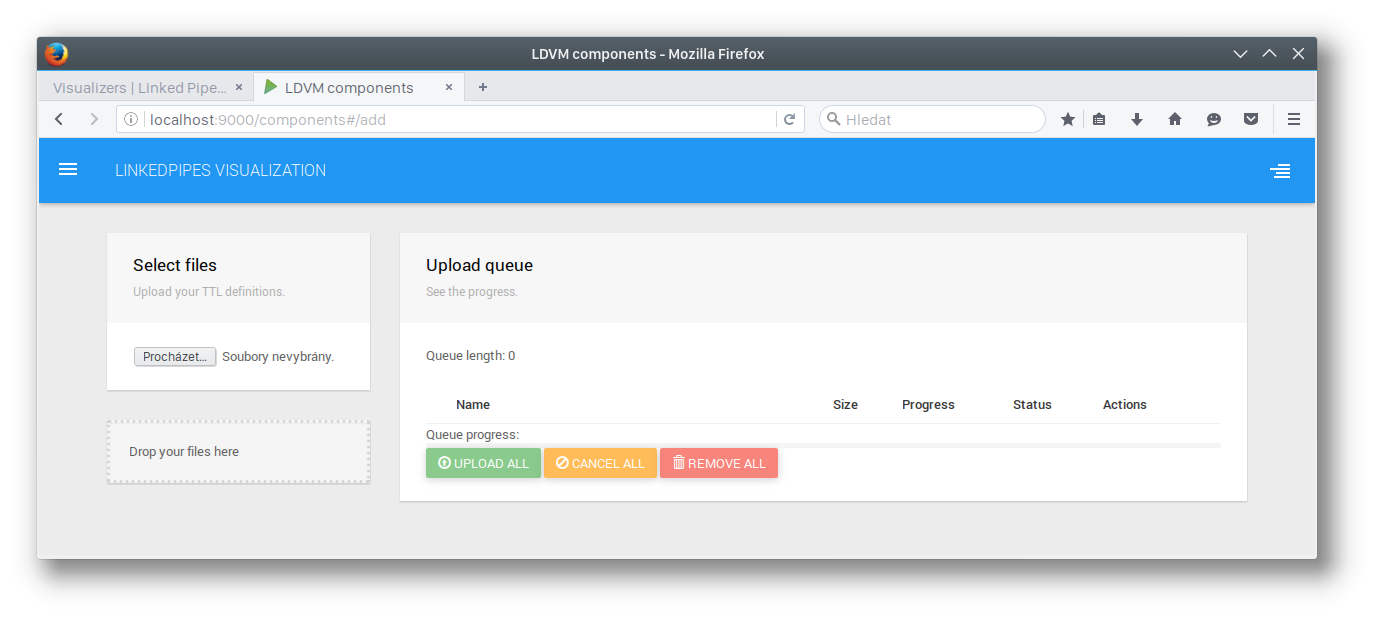
\includegraphics[width=145mm]{img/05_upload_component_definition.png}
	\caption{LinkedPipes Visualization: Upload component definition}
    \label{fig:upload_component_definition}
\end{figure}

Once this is done, the \emph{discovery} algorithm is able to utilize this new \emph{visualizer component} when discovering pipelines. If you now ran the \emph{discovery} inside LinkedPipes Visualization on a data set containing some graph data, it should find a \emph{pipeline} ending with this \emph{visualizer component}. Now we need to implement the corresponding \emph{visualizer plugin} for our \emph{application generator}.

\subsection{Frontend module}
\label{sec:implementation:integrating-visualizer:2}

As the first thing, we need to choose a unique short name for our \emph{visualizer}. When creating the RDF definition, we used the name \texttt{graph} as a RDF prefix. We will stick to this name.

A \emph{visualizer} has its own module in the \texttt{javascripts/modules/visualizers} folder. So we start by creating the appropriate module folder called \texttt{graph} and putting the file \texttt{prefix.js} into it.

\begin{verbatim}
import createPrefixer from '../../../misc/createPrefixer'

export const MODULE_PREFIX = 'graph';
export default createPrefixer(MODULE_PREFIX);
\end{verbatim}

As explained before, we will use the module name as a prefix for all our Redux \emph{actions} (or rather the prefix and the module name will be used as the \emph{visualizer} name). In this case, the prefix will also become part of the \emph{configurator} URL. Note that this is the actual and the only one \emph{source of truth} for the \emph{visualizer} name. The \texttt{MODULE\_PREFIX} value will be used when registering the plugin to the \emph{application generator}.

From now on, all paths will be relative to the \emph{visualizer} module (located at \texttt{javascripts/modules/visualizers/graph}).

\subsection{Configurator user interface}
\label{sec:implementation:integrating-visualizer:configurator}

The \emph{configurator} interfaces are part of the main \emph{platform} bundle. That means that while configuring his applications, the user never leaves the \emph{platform} SPA and the transitions between screens are always very smooth as complete page reloads are not necessary.

The integration is implemented through the router. The \emph{configurator} interface of every \emph{visualizer} defines its own routes that are registered to the \emph{platform} routes. Let us start with the main \texttt{Configurator} component defined in \texttt{pages/Configurator.js} (on Figure \ref{fig:configurator} the blurred out part corresponds to the \texttt{Configurator} component).

\begin{verbatim}
import React, { Component, PropTypes } from 'react'

class Configurator extends Component {
  render() {
    return (
      <p>This is the graph visualizer configurator.</p>
    )
  }
}
export default Configurator;
\end{verbatim}

Now we create the routes file (\texttt{configuratorRoutes.js}) with the following content:

\begin{verbatim}
import React from 'react'
import { Route } from 'react-router'
import Configurator from './pages/Configurator'
import { MODULE_PREFIX } from './prefix'

export default function createRoutes(dispatch) {
  return (
    <Route component={Configurator} path={MODULE_PREFIX} />
  );
}
\end{verbatim}

Note that we used the \texttt{MODULE\_PREFIX} as the route path.

In the final step, we register our routes. That is done in \texttt{../routes.js} (one level higher, in the parent \texttt{visualizers} module). First we have to import the routes in the file header.

\begin{verbatim}
import graphRoutes from './graph/configuratorRoutes'
\end{verbatim}

Then we need to find the right place in the file and add our routes there. The spot is clearly marked with \texttt{***Here*** you register all visualizer configurator routes} and contains a list of currently registered \emph{configurator} routes. We just need to add another line for our \texttt{graph} visualizer.

\begin{verbatim}
// ***Here*** you register all visualizer configurator routes

routeFactory.register(dataCubeRoutes);
routeFactory.register(googleMapsRoutes);
routeFactory.register(chordRoutes);
routeFactory.register(graphRoutes); // We added this line
\end{verbatim}

That is it. The last remaining step is to link the LDVM \emph{visualizer component} to this module but we will do that later. An actual URL pointing to this \emph{configurator}  could look like this: \texttt{/appgen/app/8/graph}. The number \texttt{8} is the application ID that is being configured (e.g. if the user selects this application for configuration, he is redirected to this URL). In case the \emph{visualizer} name in the URL does not correspond to the selected application (for example when the user forces a different value to the URL), the user is automatically redirected to the correct \emph{configurator}.

If the reader is asking why the \emph{configurator} is part of the URL when this information can be derived directly from the application ID, we would kindly refer to Subsection \ref{sec:implementation:design-choices:integration}.

Before moving to the next step, we will slightly improve the \texttt{Configurator} component.

\begin{verbatim}
import React, { Component, PropTypes } from 'react'
import BodyPadding from '../../../../components/BodyPadding'
import { Application } from '../../../app/models'
import { Visualizer } from '../../../core/models'

class Configurator extends Component {
  static propTypes = {
    application: PropTypes.instanceOf(Application).isRequired,
    visualizer: PropTypes.instanceOf(Visualizer).isRequired
  };

  render() {
    const { application, visualizer } = this.props;
    return (
      <BodyPadding>
        <p>This is the graph visualizer configurator.</p>
        <p>{application.name}</p>
        <p>{visualizer.title}</p>
      </BodyPadding>
    )
  }
}

export default Configurator;
\end{verbatim}

The objects representing the selected application and visualizer are  for your convenience automatically injected using \texttt{props} to the \texttt{Configurator} component (but they are available from the \emph{state} at any time). Here we just use them to print their names. We also used the \texttt{BodyPadding} component to add the standard padding around the text.

\subsection{Application user interface}
\label{sec:implementation:integrating-visualizer:4}

As explained, the \emph{application} interface of each \emph{visualizer} lives in a standalone JavaScript bundle. The \emph{application} interface that we are about to implement will support embedding. It will run in two different modes. There will be the default \emph{standalone} mode which besides the visualization itself will also display the application name and description. It will be accessible on the default root \texttt{/} URL. Then there will be the \emph{embed} mode containing just the visualization. It will be accessible on the \texttt{/embed} URL.

We will start similarly to the \emph{configuration} interface by defining the main \texttt{Application} component in \texttt{components/Application.js}. Note that it is no longer in the \texttt{pages} folder.

\begin{verbatim}
import React, { Component, PropTypes } from 'react'
import BodyPadding from '../../../../components/BodyPadding'
import { Application as ApplicationModel } from '../../../app/models'
import { Visualizer } from '../../../core/models'

class Application extends Component {
  static propTypes = {
    application: PropTypes.instanceOf(ApplicationModel).isRequired,
    visualizer: PropTypes.instanceOf(Visualizer).isRequired,
    embed: PropTypes.bool
  };

  render() {
    const { application, visualizer, embed } = this.props;
    return (
      <BodyPadding>
        <p>This is the graph visualizer application.</p>
        <p>It runs in {embed ? 'embed' : 'standalone'} mode</p>
        <p>{application.name}</p>
        <p>{visualizer.title}</p>
      </BodyPadding>
    )
  }
}

export default Application;
\end{verbatim}

The content is at this moment almost identical to the \texttt{Configurator} component. It just displays the current application name and visualizer title. But this time it also shows whether it runs in the \emph{standalone} or \emph{embed} mode. 

Now for each mode we will need a different component as each mode lives at a different URL. Let us start with \texttt{pages/Embed.js}.

\begin{verbatim}
import React from 'react'
import Application from '../components/Application'

export default props => <Application embed {...props} />
\end{verbatim}

And now \texttt{pages/Standalone.js}.

\begin{verbatim}
import React, { PropTypes } from 'react'
import Application from '../components/Application'
import ApplicationHeader from '../../../app/components/ApplicationHeader'

const Standalone = props => (
  <div>
    <ApplicationHeader {...props} />
    <Application {...props} />
  </div>
);

export default Standalone;
\end{verbatim}

Note that both times, we re-use the \texttt{Application} component but in the \emph{standalone} mode we add a standard header that renders the application name and description. What remains is to tie it all together with routes definition. We put it to \texttt{applicationRoutes.js} just next to \texttt{configuratorRoutes.js}.

\begin{verbatim}
import React from 'react'
import { Route, IndexRoute } from 'react-router'
import ApplicationLoader from '../../app/pages/ApplicationLoader'
import NotFound from '../../platform/pages/NotFound'
import Standalone from './pages/Standalone'
import Embed from './pages/Embed'

export default function createRoutes(dispatch) {
  return (
    <Route component={ApplicationLoader} path='/'>
      <IndexRoute component={Standalone} />
      <Route component={Embed} path='embed' />
      <Route component={NotFound} path='*' />
    </Route>
  );
}
\end{verbatim}

Note that the top level path is directly \texttt{/}. This routes definition will not be registered to any existing route hierarchy. It contains the complete routing information for this standalone SPA. For this reason, we use the \texttt{ApplicationLoader} as the top level component to load the application from the server first. This has been done automatically for us in the case of \emph{configurator} interface.
 
In the final step, we need to add a new Webpack \emph{entry point}. We create a file \texttt{javascripts/entries/graph.js} (this time relative to the \texttt{assets} folder) with the following content. 

\begin{verbatim}
import createRoutes from '../modules/visualizers/graph/applicationRoutes'
import initEntry from '../misc/initEntry'

initEntry(createRoutes);
\end{verbatim}

We have to make sure to import the correct routes definition and also that the file name corresponds to the \emph{visualizer} name. Webpack will pick up this new \emph{entry point} automatically (if you are running Webpack in the watch mode, you need to restart it) and generate a new JavaScript bundle of the same name.

\subsection{Linking LDVM component to the plugin}
\label{sec:implementation:integrating-visualizer:5}

In this step, we will link the LDVM \emph{visualizer component} and the \emph{visualizer} plugin together. That is done through the \emph{application generator} user interface (not LinkedPipes Visualization interface this time).

We need to sign in to the \emph{application generator} with an administrator account. We navigate to the \textbf{Dashboard}, select \textbf{Visualizers} and click the button \textbf{Add visualizer}. A dialog window will appear, containing a list of unused available LDVM \emph{visualizer components}. We select \textbf{Graph Visualizer} (which is the name we provided in the RDF definition)  and click \textbf{Add visualizer}. The new \emph{visualizer} should appear in the table. We click its name to open a configuration dialog window (Figure \ref{fig:edit-visualizer}). We ignore the first two fields as they are related to LinkedPipes Visualization. The most important field is the name as it determines which bundle to load for the \emph{application} interface and to which \emph{configurator} URL to redirect. We fill in \texttt{graph}. It is crucial that this value corresponds to the \emph{visualizer} module name, the prefix and the \emph{entry point} name. We also recommend filling in the \emph{visualizer} icon for better user experience. Currently, Material Icons \footnote{https://design.google.com/icons/} collection is used. We chose the \texttt{device\_hub} icon.

\begin{figure}
	\centering
	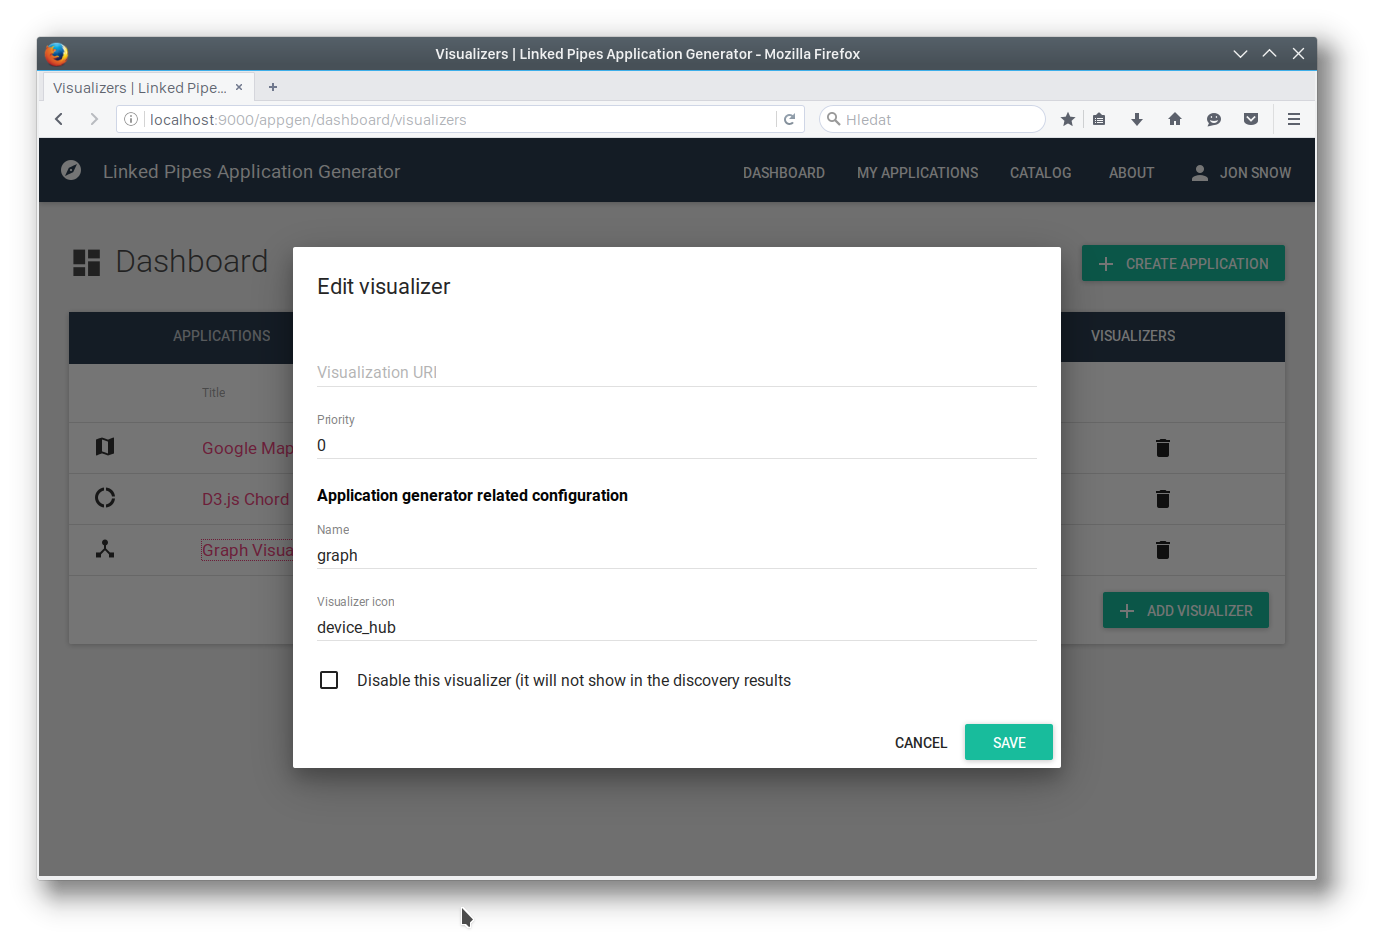
\includegraphics[width=140mm]{img/05_edit_visualizer.png}
	\caption{Configuration dialog window of a \emph{visualizer}.} 
	\label{fig:edit-visualizer}
\end{figure}
This was the last mandatory step. At this moment, the \emph{visualizer} (even though it does not do anything) should be working, i.e., it should be possible to create a new application using this \emph{visualizer} from a data set containing graph data.

\subsection{Scala backend}
\label{sec:implementation:integrating-visualizer:6}

Surprisingly enough, we did not have to touch the Scala backend to register our new \emph{visualizer}. Technically speaking, it is really not necessary but only until the very moment when we need the \emph{visualizer} to actually \textit{do something useful}. That typically involves fetching and extracting the RDF data produced by the \emph{pipeline}. For that we do need the backend.

In this subsection, we will simply prepare the controller that will be handling our client requests.

\begin{verbatim}
package controllers.appgen.api.visualizers
import scaldi.Injector

class GraphVisualizerApiController(implicit inj: Injector) extends VisualizerApiController { }
\end{verbatim}

The package information clearly says where this class should belong. The \texttt{VisualizerApiController} will provide us with some utilities that will come handy later.

\subsection{Extracting RDF data from the pipeline evaluation}
\label{sec:implementation:integrating-visualizer:extracting-rdf}

We said that our \emph{visualizer} would show the number of vertices and edges in the graph. For us that means that we need to access the RDF data produced by the \emph{pipeline}, extract this information from it, send it to the client and then display it on the screen. We start with accessing the RDF data. Note that in this part, we are utilizing the LinkedPipes Visualization API for working with RDF data.

Since it is RDF data, we will use SPARQL queries to fetch the information we need. 

\begin{verbatim}
package model.rdf.sparql.rgml.query
import model.rdf.sparql.query.SparqlQuery

class GraphQuery extends SparqlQuery {

  def get: String =
    """
      | PREFIX rdf: <http://www.w3.org/1999/02/22-rdf-syntax-ns#>
      | PREFIX rgml: <http://purl.org/puninj/2001/05/rgml-schema#>
      |
      | SELECT ?directed ?nodeCount ?edgeCount WHERE {
      |   ?graph
      |     rdf:type rgml:Graph ;
      |     rgml:directed ?directed .
      |
      |   { SELECT (COUNT(*) AS ?nodeCount) WHERE { ?edge rdf:type rgml:Node . } }
      |   { SELECT (COUNT(*) AS ?edgeCount) WHERE { ?edge rdf:type rgml:Edge . } }
      | }
      | LIMIT 1
    """
      .stripMargin
}
\end{verbatim}

This is the recommended way of representing SPARQL queries in our Scala code. As you can see, the query counts all the edges and vertices (which are called \emph{nodes} in the RGML vocabulary) and also fetches the information about whether the graph is directed or not.

The result of this query will be represented using a simple Scala case class. For simplicity, we just call it \texttt{Graph}.

\begin{verbatim}
package model.rdf.sparql.rgml

case class Graph(directed: Boolean, nodeCount: Int, edgeCount: Int)
\end{verbatim}

Now we need a tool that will convert the fetched RDF data into this case class. Such a tool is called an \emph{extractor}.

\begin{verbatim}
package model.rdf.sparql.rgml.extractor

import model.rdf.extractor.QueryExecutionResultExtractor
import model.rdf.sparql.rgml.Graph
import model.rdf.sparql.rgml.query.GraphQuery
import org.apache.jena.query.QueryExecution


class GraphExtractor extends QueryExecutionResultExtractor[GraphQuery, Graph] {

  def extract(input: QueryExecution): Option[Graph] = {

    try {
      val resultSet = input.execSelect
      val solution = if (resultSet.hasNext) Some(resultSet.next) else None

      solution map { solution => Graph(
        solution.getLiteral("directed").getBoolean,
        solution.getLiteral("nodeCount").getInt,
        solution.getLiteral("edgeCount").getInt)
      }
    } catch {
      case e: org.apache.jena.sparql.engine.http.QueryExceptionHTTP => {
        None
      }
    }
  }
}
\end{verbatim}

Apache Jena \footnote{https://jena.apache.org/} framework is used internally to work with RDF data. Our SPARQL query is a SELECT query which means that the results will be in a form of tabular data (i.e., a set of rows where each row contains the same columns). We assume that the data set contains only one graph, so we take the first row (if available) and convert it to the \texttt{Graph} case class.

Finally, we need something that will execute the query and apply the extractor on the results.

\begin{verbatim}
package model.rdf.sparql.rgml
//  ...imports

class RgmlService(implicit val inj: Injector) extends RgmlService with Injectable {
  var sparqlEndpointService = inject[SparqlEndpointService]

  def graph(evaluation: PipelineEvaluation)(implicit session: Session): Option[Graph] = {
    sparqlEndpointService.getResult(
      evaluationToSparqlEndpoint(evaluation),
      new GraphQuery(),
      new GraphExtractor())
  }
\end{verbatim}

As you can see, we defined \texttt{RgmlService} with the \texttt{graph} method. The \emph{pipeline evaluation} does not directly contain the data but rather points where the data are (i.e., it specifies the SPARQL endpoint and concrete named graphs with the data). We use \texttt{SparqlEndpointService} to access it and extract our graph from it. The function \texttt{evaluationToSparqlEndpoint} is just an utility that we omitted to keep the code short. % TODO: add it to a trait

You might have noticed that we put all the files in the same package \texttt{model.rdf.sparql.rgml}. What we are doing is that we are adding support for RGML vocabulary to the LinkedPipes Visualization code base in a way that anyone can use it for their \emph{visualizers}, i.e., it is \emph{visualizer} independent.

For the \texttt{RgmlService} to work properly, it has to be registered to the Dependency Injection container in \texttt{model.rdf.RdfModule}.

Let us now move from the \emph{Model} layer to the \emph{Controller} layer. We will extend the controller we defined earlier with an action that will use this service to fetch the graph information and send it to the client serialized to JSON.

\begin{verbatim}
class GraphVisualizerApiController(implicit inj: Injector) extends VisualizerApiController {
  val rgmlService = inject[RgmlService]

  def getGraph(id: Long) = RestAsyncAction[EmptyRequest] { implicit request => json =>
    withEvaluation(ApplicationId(id)) { evaluation =>
      val graph = rgmlService.graph(evaluation)
      Future(Ok(SuccessResponse(data = Seq("graph" -> graph))))
    }
  }
}
\end{verbatim}

The \texttt{getGraph} action is mapped to a URL with a single parameter \texttt{id} (the URL mappings are defined in the file \texttt{src/conf/routes}, relative to the code base root). The \texttt{id} is an application ID. We use the \texttt{withEvaluation()} helper to load the appropriate \emph{pipeline evaluation}, then we fetch the graph using our \texttt{RgmlService} and send it to the client in a \texttt{SuccessReponse}. The API is designed to support \texttt{Futures} in case the requests are expected to be computationally heavy and need to be performed asynchronously. This is not our case but we need to follow the API. That is why the response is wrapped by the \texttt{Future} call.

In order for the \texttt{Graph} case class to be automatically converted to JSON, we need to define an \emph{implicit converter}. We can do it by adding following lines to \texttt{controllers.api.JsonImplicits} and import it to the controller:

\begin{verbatim}
implicit val graphWrites = Json.writes[Graph]
\end{verbatim}

\subsection{Making asynchronous requests from the client}
\label{sec:implementation:integrating-visualizer:8}

Everything is prepared on the server-side. Now comes the client. When the application loads, we will make an synchronous HTTP request to fetch the graph information. Once we receive it, we store it in the \emph{state} and show it on the screen.

We start by creating a JavaScript counterpart for the Scala \texttt{Graph} case class. Note that once again, all paths are relative to the \emph{visualizer} module. Also to keep the text shorter, we will just state the file name at the beginning of each snippet.

\begin{verbatim}
// models.js

import { Record } from 'immutable';

export const Graph = Record({
  directed: false,
  nodeCount: 0,
  edgeCount: 0
});
\end{verbatim}

We create a simple explicit wrapper for the asynchronous HTTP request.

\begin{verbatim}
// api.js

import rest from '../../../misc/rest'

export async function getGraph(applicationId) {
  const result = await rest('graphVisualizer/getGraph/' + applicationId, {});
  return result.data.graph;
}
\end{verbatim}

The keywords \texttt{async/await} are just syntactical sugar around \texttt{Promises}. They allow us to write \emph{asynchronous} code in a \emph{synchronous} manner.

Now we will define a new \emph{duck} that will handle and provide API for fetching the graph information (using an \emph{action}), storing it in the \emph{state} (using a \emph{reducer}) and selecting it from the \emph{state} (using a \emph{selector}). Let us start with \emph{actions} (we will always put the currently required \texttt{imports} to the top of each code snippet; in the actual file they will all be together at the beginning).

\begin{verbatim}
// ducks/graph.js

import createAction from '../../../../misc/createAction'
import withApplicationId from '../../../app/misc/withApplicationId'
import prefix from '../prefix'
import * as api from '../api'

// Actions

export const GET_GRAPH = prefix('GET_GRAPH');
export const GET_GRAPH_START = GET_GRAPH + '_START';
export const GET_GRAPH_ERROR = GET_GRAPH + '_ERROR';
export const GET_GRAPH_SUCCESS = GET_GRAPH + '_SUCCESS';
export const GET_GRAPH_RESET = GET_GRAPH + '_RESET';

export function getGraph() {
  return withApplicationId(id => {
    const promise = api.getGraph(id);
    return createAction(GET_GRAPH, { promise });
  })
}

export function getGraphReset() {
  return createAction(GET_GRAPH_RESET);
}
\end{verbatim}

The \emph{action creator} \texttt{getGraph()} first uses the \texttt{withApplicationId} utility to extract the application ID from the \emph{state} and then calls the API function to make the HTTP request to the server. The request result is represented using a \texttt{Promise} which is \emph{dispatched} as an action payload. There is a \emph{redux middleware} running in the background that detects the \texttt{Promise}, dispatches \texttt{GET\_GRAPH\_START} and then depending on the result either \texttt{GET\_GRAPH\_ERROR} or \texttt{GET\_GRAPH\_SUCCESS}. We do not actually have to define all the \emph{action} constants but it is good practice (note that we used the module prefixer). The \texttt{START}, \texttt{ERROR}, \texttt{SUCCESS} and \texttt{RESET} suffixes are defined by a convention.

In the next step, we will implement the reducer that will store the graph.

\begin{verbatim}
// ducks/graph.js

import { GET_APPLICATION_START } from '../../../app/ducks/application'
import { Graph } from '../models'

// Reducer

const initialState = new Graph();

export default function graphReducer(state = initialState, action) {
  switch (action.type) {
    case GET_APPLICATION_START:
    case GET_GRAPH_RESET:
      return initialState;

    case GET_GRAPH_SUCCESS:
      return new Graph(action.payload);
  }

  return state;
};
\end{verbatim}

Note that the initial state is a valid (but empty) \texttt{Graph} object. That means that we can work with this object safely at any time (it will not be \texttt{null}).

Finally, we will create \emph{selectors} that will allow us to easily extract the \texttt{Graph} from the state.

\begin{verbatim}
// ducks/graph.js

import { createSelector } from 'reselect'
import { createPromiseStatusSelector } from '../../../core/ducks/promises'
import moduleSelector from '../selector'

// Selectors

export const graphStatusSelector = createPromiseStatusSelector(GET_GRAPH);
export const graphSelector = createSelector([moduleSelector], state => state.graph);
\end{verbatim}

The first one selects the HTTP request status, the second one selects the actual graph. Now we need to integrate both the \emph{selectors} and the \emph{reducer} to the \emph{state} hierarchy.

\begin{verbatim}
// reducer.js

import { combineReducers } from 'redux';
import graph from './ducks/graph'

const rootReducer = combineReducers({
  graph
});

export default rootReducer;
\end{verbatim}

This is the root \emph{reducer} of the \emph{visualizer} module that combines all other reducers in the module together. It has to be registered to the parent reducer in the parent module.

\begin{verbatim}
import { combineReducers } from 'redux';
import googleMaps from './googleMaps/reducer'
import chord from './chord/reducer'
import graph from './graph/reducer'

const rootReducer = combineReducers({
  googleMaps,
  chord,
  graph // We added this line
});
export default rootReducer;
\end{verbatim}

We have to do the same for the \emph{selectors} as well.

\begin{verbatim}
// selector.js

import { createSelector } from 'reselect'
import parentSelector from '../selector'
import { MODULE_PREFIX } from './prefix'

export const moduleSelector = createSelector(
  [parentSelector],
  parentState => parentState[MODULE_PREFIX]
);
export default moduleSelector;
\end{verbatim}

You might have noticed that we already used this file in \texttt{ducks/graph.js}. What is important here is that the key we use to register the \emph{reducer} is the same as the key we use in the \emph{selector}. They both access the same data in the same \emph{state} object (\emph{reducer} for updating, \emph{selector} for reading).

Now that everything is ready, we create a simple component that will fetch and display the graph information. We start with the component life cycle methods.

\begin{verbatim}
// components/GraphLoader.js

import React, { Component, PropTypes } from 'react'
import { getGraph, getGraphReset } from '../ducks/graph'

class GraphLoader extends Component {
  componentWillMount() {
    const { dispatch } = this.props;
    dispatch(getGraph());
  }
  
  componentWillUnmount() {
    const { dispatch } = this.props;
    dispatch(getGraphReset());
  }
}
\end{verbatim}

Once the component appears on the screen, it will initiate the request. When it is about to leave, it will reset the \emph{state} 
(clean up after itself). We will \emph{connect} the component to Redux and inject the data that we need.

\begin{verbatim}
// components/GraphLoader.js

import { connect } from 'react-redux'
import { createStructuredSelector } from 'reselect'
import { getGraph, getGraphReset, graphSelector, graphStatusSelector } from '../ducks/graph'

const selector = createStructuredSelector({
  graph: graphSelector,
  status: graphStatusSelector
});

export default connect(selector)(GraphLoader);
\end{verbatim}

It is always a good practice to explicitly define the \texttt{propTypes}.

\begin{verbatim}
// components/GraphLoader.js

import { PromiseStatus } from '../../../core/models'
import { Graph } from '../models'

class GraphLoader extends Component {
  static propTypes = {
    dispatch: PropTypes.func.isRequired,
    graph: PropTypes.instanceOf(Graph).isRequired,
    status: PropTypes.instanceOf(PromiseStatus).isRequired
  };
  
  // ...
}
\end{verbatim}

Lastly, we implement the \texttt{render} method.

\begin{verbatim}
// components/GraphLoader.js

import PromiseResult from '../../../core/components/PromiseResult'

class GraphLoader extends Component {
  // ...
  
  render() {
    const { graph, status } = this.props;

    if (!status.done) {
      return <PromiseResult status={status} loadingMessage="Loading base graph info..." />
    }

    return (
      <div>
        <p><strong>Graph info</strong></p>
        <p>Node count: {graph.nodeCount}</p>
        <p>Edge count: {graph.edgeCount}</p>
        <p>Directed: {graph.directed ? 'yes' : 'no'}</p>
      </div>
    )
  }
\end{verbatim}

The \texttt{status.done} value changes to \texttt{true} only if the request successfully finishes (i.e., the \emph{action} \texttt{GET\_GRAPH\_SUCCESS} is \emph{dispatched}). Therefore once the value is \texttt{true} we can be sure that the graph information is correctly stored in the \emph{state}. Before this happens, we display the \texttt{PromiseResult} component which shows a nice loading bar and if the request fails, it displays an error message. 

What remains to be done is to add the \texttt{GraphLoader} component to the \emph{configurator} and \emph{application} user interface.

\begin{verbatim}
// pages/Configurator.js

import GraphLoader from '../containers/GraphLoader'

class Configurator extends Component {
  // ...

  render() {
    const { application, visualizer } = this.props;
    return (
      <BodyPadding>
        <p>This is the graph visualizer configurator.</p>
        <p>{application.name}</p>
        <p>{visualizer.title}</p>
        <GraphLoader />
      </BodyPadding>
    )
  }
}
\end{verbatim}

\begin{verbatim}
// components/Application.js

import GraphLoader from '../containers/GraphLoader'

class Application extends Component {
  // ...

  render() {
    const { application, visualizer, embed } = this.props;
    return (
      <BodyPadding>
        <p>This is the graph visualizer application.</p>
        <p>It runs in {embed ? 'embed' : 'standalone'} mode</p>
        <p>{application.name}</p>
        <p>{visualizer.title}</p>
        <GraphLoader />
      </BodyPadding>
    )
  }
}
\end{verbatim}

\subsection{Saving and loading application configuration}
\label{sec:implementation:integrating-visualizer:configuration}

The framework provides an optional solution for saving and loading the application configuration easily. The idea is very simple yet powerful. The configuration consists of different bits and pieces of the \emph{state}. To save the configuration, we just serialize those bits and pieces into JSON and save it on the server. To load the configuration, we fetch it from the server, unserialize it from JSON and let the \emph{reducers} to update the \emph{state}.

The configuration contains parts that are \emph{visualizer} specific and parts that are common for all \emph{visualizers} and we have to make sure that they both are saved and loaded properly together.

We starting by creating a \texttt{dirty} \emph{duck} with a \emph{reducer} that will simply indicate with a boolean value whether the configuration has changed.

\begin{verbatim}
// ducks/dirty.js

import { createSelector } from 'reselect'
import moduleSelector from '../selector'
import { createDirtyReducer } from '../../../app/ducks/dirty'

// Reducer

const actions = [ ];

export default createDirtyReducer(actions);

// Selectors

export const dirtySelector = createSelector([moduleSelector], state => state.dirty);
\end{verbatim}

The \texttt{actions} constant contains the list of \emph{actions} that change the state. Whenever such an \emph{action} is dispatched, the \emph{dirty} status changes to \texttt{true}. The \emph{reducer} has to be properly registered in the module root \emph{reducer}.

The next \emph{duck} will define the \emph{actions} for saving and loading the configuration. They will be created using framework factories that will ensure proper integration.

\begin{verbatim}
import prefix from '../prefix'
import moduleSelector from '../selector'
import { createPromiseStatusSelector } from '../../../core/ducks/promises'
import { 
  createGetConfiguration, createGetConfigurationReset, createSaveConfiguration 
} from '../../../app/ducks/configuration'

// Actions

export const SAVE_CONFIGURATION = prefix('SAVE_CONFIGURATION');
export const SAVE_CONFIGURATION_START = SAVE_CONFIGURATION + '_START';
export const SAVE_CONFIGURATION_ERROR = SAVE_CONFIGURATION + '_ERROR';
export const SAVE_CONFIGURATION_SUCCESS = SAVE_CONFIGURATION + '_SUCCESS';

export const GET_CONFIGURATION = prefix('GET_CONFIGURATION');
export const GET_CONFIGURATION_START = GET_CONFIGURATION + '_START';
export const GET_CONFIGURATION_ERROR = GET_CONFIGURATION + '_ERROR';
export const GET_CONFIGURATION_SUCCESS = GET_CONFIGURATION + '_SUCCESS';
export const GET_CONFIGURATION_RESET = GET_CONFIGURATION + '_RESET';

// Selectors

export const saveConfigurationStatusSelector = createPromiseStatusSelector(SAVE_CONFIGURATION);
export const getConfigurationStatusSelector = createPromiseStatusSelector(GET_CONFIGURATION);

export const configurationSelector = createSelector(
  [moduleSelector],
  state => ({  })
);

// Actual actions created using factories
export const saveConfiguration = 
  createSaveConfiguration(SAVE_CONFIGURATION, configurationSelector);
export const getConfiguration = 
  createGetConfiguration(GET_CONFIGURATION);
export const getConfigurationReset = 
  createGetConfigurationReset(GET_CONFIGURATION_RESET);
\end{verbatim}

The \texttt{configurationSelector} defines what parts of the \emph{state} should get into the configuration. At this moment, the \emph{state} just contains the graph information which is available from the \emph{pipeline evaluation}. There is no point in making that part of the configuration. When the configuration is loaded from the server, the \emph{action} \texttt{GET\_CONFIGURATION\_SUCCESS} is \emph{dispatched} with the configuration in the payload. The \emph{reducers} can simply listen to this action and extract from the payload the information that is relevant to them. As the \emph{action} is prefixed, it will not cause any conflicts.

The next step of integration is the \textbf{Save} button. Once again we use a framework factory to create the button component. The button is interactive which means it automatically indicates whether the configuration needs to be saved (using the \texttt{dirty} information) or whether the saving is in progress. We will add the button to the \texttt{Configurator} component.

\begin{verbatim}
import React, { PropTypes } from 'react'
import { saveConfiguration, saveConfigurationStatusSelector } from '../ducks/configuration'
import { dirtySelector } from '../ducks/dirty'

import createSaveButton from '../../../app/containers/createSaveButton'

export default createSaveButton(
  saveConfiguration,
  saveConfigurationStatusSelector,
  dirtySelector);
\end{verbatim}

In the final step, we need to load the configuration when the \emph{configurator} (or \emph{application}) initiates.

\begin{verbatim}
// pages/Configurator.js

import { getConfiguration, getConfigurationReset } from '../ducks/configuration'

class Configurator extends Component {
  // ...

  componentWillMount() {
    const { dispatch } = this.props;
    dispatch(getConfiguration());
  }

  componentWillUnmount() {
    const { dispatch } = this.props;
    dispatch(getConfigurationReset());
  }
  
  // ...
}
\end{verbatim}

Similarly, we would load the configuration in the \texttt{Application} component.

As a concrete example, we will let the user to edit graph label. To keep this subsection short, we will utilize one of the available framework utilities, custom label editor (Figure~\ref{fig:scenario-08-custom-label-editor}). This editor allows the user to specify alternative labels for RDF resources. Each RDF resource is identified with a URI. Unfortunately, we do not have the graph URI but for simplicity, we will just make up one.

\begin{verbatim}
// pages/Configurator.js

import EditableLabel from '../../../app/containers/EditableLabel'
import SaveButton from '../containers/SaveButton'

class Configurator extends Component {
  // ...

  render() {
    const { application, visualizer } = this.props;
    return (
      <BodyPadding>
        <h3><EditableLabel uri="http://example.org/graph" label="Unnamed graph" /></h3>
        <p>This is the graph visualizer configurator.</p>
        <p>{application.name}</p>
        <p>{visualizer.title}</p>
        <GraphLoader />
        <SaveButton />
      </BodyPadding>
    )
  }
}
\end{verbatim}

That is it. If we now click the \textbf{More} button in the upper right corner of the \emph{configurator} interface and then select \textbf{Edit labels}, a pencil icon will appear next to the graph name (which will be "Unnamed graph" by default). Clicking that icon will open a dialog where we can define a language dependent values for this resource. By clicking \textbf{Save}, we update the \emph{state} and we can immediately see the change on the screen. By clicking \textbf{Save changes}, we save the changes to the server (the custom labels are part of the common configuration which means that it is automatically taken care of). We now have to add the \texttt{EditableLabel} component to the \texttt{Application} component as well to get it working in the \emph{application} interface.

\subsection{Final notes}
\label{sec:implementation:integrating-visualizer:final-notes}

You might have noticed that we have repeated a lot of work for the \emph{application} and \emph{configurator} interface and their components are nearly identical. Firstly, in a more complex \emph{visualizer} those two interfaces would differ significantly more. Secondly, thanks to the React nature it is always very easy to refactor the code, put the shared aspects into a single component and then re-use it. No doubt that some of these features could have been implemented more simply but you should consider this a starting point from which you can start extending and building your \emph{visualizer}.

Also some parts might have seemed excessively verbose. For example, when we defined all the \emph{action type} constants for saving and loading the configuration (Subsection \ref{sec:implementation:integrating-visualizer:configuration}). To an extent this verbosity is caused by the development stack. In this particular case, it is up to the developer whether he decides to define all \emph{action types} that might occur as part of good practice, or to define just those that he actually needs. We prefer defining all \emph{action types} as it explicitly describes what can happen in the application.

The result of our work can be seen on Figure \ref{fig:graph-visualizer}. For more complex examples we suggest the user to check out the full implementations of the two completed visualizers, the D3.js Chord Visualizer and Google Maps Visualizer (both will be described later).

\begin{figure}
	\centering
	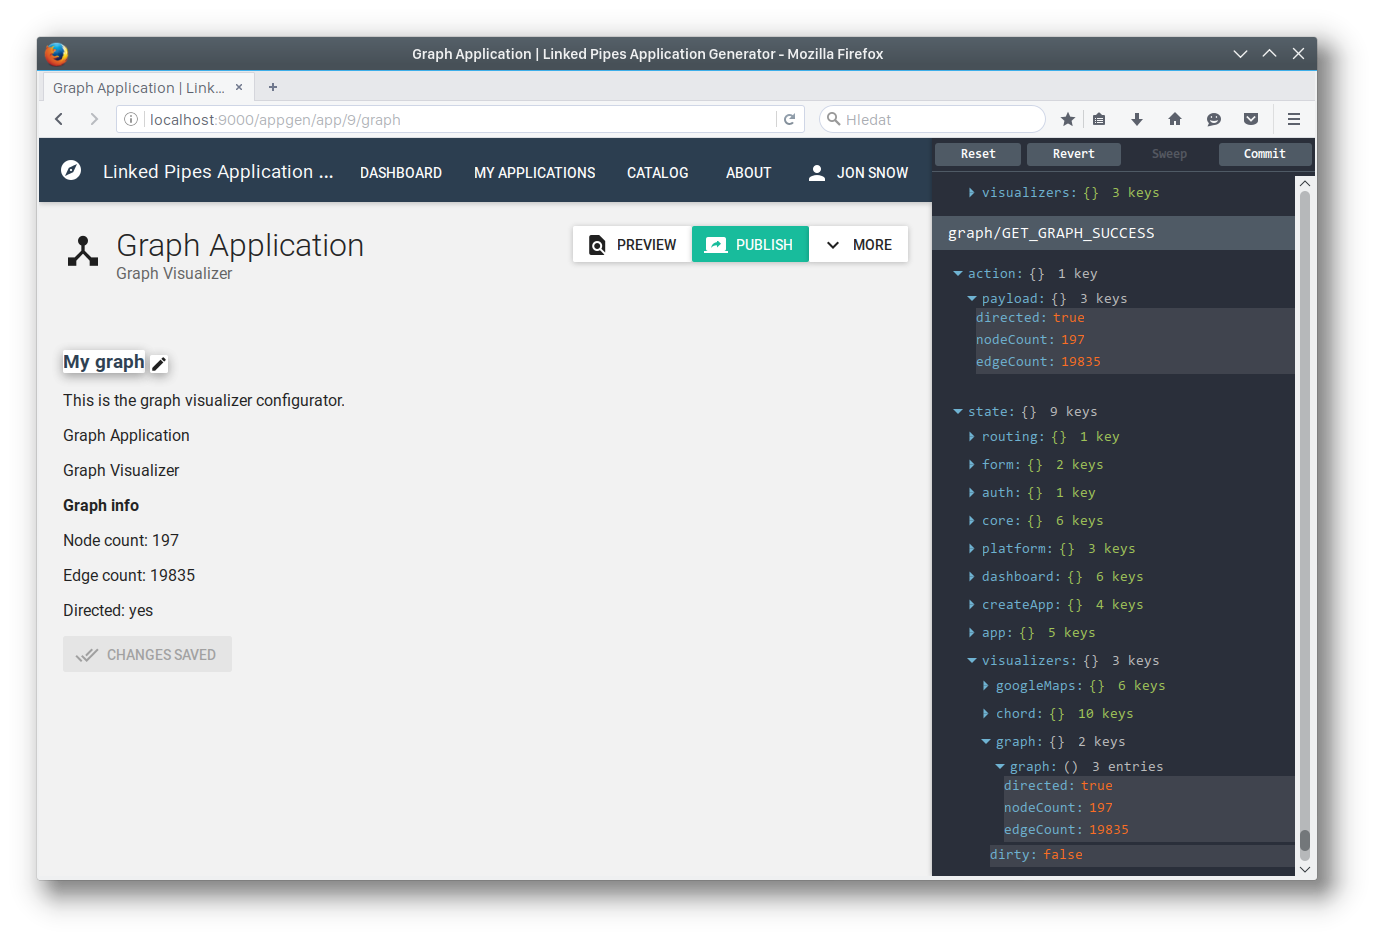
\includegraphics[width=145mm]{img/05_graph_visualizer}
	\caption{\emph{Configurator} interface of the sample Graph Visualizer. The Redux development sidebar is enabled showing the \emph{state}.}
    \label{fig:graph-visualizer}
\end{figure}

\section{Advanced framework features}

While we were demonstrating how a new \emph{visualizer} can be integrated into our \emph{application generator}, we showed couple of available features that the developer can use to speed up the process. Namely, we described the prepared solution for saving and loading application configuration and we also showed how we can easily extract RDF data from the \emph{pipeline evaluation}. Here we will briefly mention couple more examples.

\subsection{Request cache}

As some requests might be quite computationally heavy, we implemented a simple caching solution for the server side. For example, this is the controller action that fetches the graph information (Subsection \ref{sec:implementation:integrating-visualizer:extracting-rdf}):

\begin{verbatim}
class GraphVisualizerApiController(implicit inj: Injector) extends VisualizerApiController {
  val rgmlService = inject[RgmlService]

  def getGraph(id: Long) = RestAsyncAction[EmptyRequest] { implicit request => json =>
    withEvaluation(ApplicationId(id)) { evaluation =>
      val graph = rgmlService.graph(evaluation)
      Future(Ok(SuccessResponse(data = Seq("graph" -> graph))))
    }
  }
}
\end{verbatim}

Making this request cached is very simple:

\begin{verbatim}
class GraphVisualizerApiController(implicit inj: Injector) extends VisualizerApiController {
  val rgmlService = inject[RgmlService]

  def getGraph(id: Long) = RestAsyncAction[EmptyRequest] { implicit request => json =>
    cached {
      withEvaluation(ApplicationId(id)) { evaluation =>
        val graph = rgmlService.graph(evaluation)
        Future(Ok(SuccessResponse(data = Seq("graph" -> graph))))
      }
    }
  }
}
\end{verbatim}

The solution works on a request level (it uses all available request information, including URL, POST data and the current user to identify the request). What is important is that the requests are cached persistently in the database which means that the cache will survive even application crashes. The solution is very basic and the point is just to demonstrate the capabilities. The default caching solution for the Play Framework is Ehcache \footnote{http://www.ehcache.org/} but that supports persistent caching only in the paid version.

\subsection{Multiple language support}
\label{sec:implementation:advanced-features:multiple-language-support}


RDF may contain values (typically labels) in multiple languages. If correctly extracted, such a value is represented using the \texttt{model.rdf.LocalizedValue} Scala case class which, serialized to JSON, looks like this:

\begin{verbatim}
{
  'variants': {
    'en': 'Czech Republic',
    'cs': 'Česká republika'
  }
}
\end{verbatim}

The frontend framework offers a simple way how to display these values.

\begin{verbatim}
import React from 'react'
import LocalizedValue from './LocalizedValue'

const Country = country => (
    <h3><LocalizedValue localizedValue={country.label} /></h3>
  );
\end{verbatim}

If the \texttt{country.label} value is in the format suggested above, the component will automatically choose the value corresponding to the language currently selected by the user (if it is available).

The problem here is to determine what languages are actually available (i.e., what languages the user can select from). As this information is not available anywhere, we use a \emph{brute force} solution to find it. In Redux, every \emph{action} is \emph{dispatched} to every \emph{reducer}. Typically, one \emph{reducer} only responds to couple of related \emph{actions} but to solve our problem, we introduced a special \emph{reducer} that responds to every \emph{action} and searches through the payloads for available languages (it is looking for the object structure suggested above). The \emph{reducer} uses a simple Depth-first search algorithm to recursively search through the whole payload.

For example, whenever we fetch something from the server, the incoming data are \emph{dispatched} as a payload of some \texttt{SUCCESS} action. Our special \emph{reducer} searches that payload and if it finds any new languages, it adds them to the \emph{state}. An updated language switch is consequently displayed to the user.

\subsection{Label dereferencing}
\label{sec:implementation:advanced-features:label-dereferencering}

It is pretty common that an RDF resource contains a label which we can display to the user. But sometimes it is not available in frontend, maybe because it was simply not fetched from the server, maybe because it is not present in the data set at all. The frontend framework offers another useful component that attempts to fix this problem.

\begin{verbatim}
import React from 'react'
import LocalizedValue from './LocalizedValue'

const Country = country => (
    <h3><Label uri={country.uri} label={country.label} /></h3>
  );
\end{verbatim}

If \texttt{country.label} is empty, the component will make a request to the server which will at first try to load the label from the \emph{pipeline evaluation} and if the label is not there, it will use a technique called \emph{dereferencing}. That involves directly accessing the resource URI using the HTTP protocol and trying to extract the label from the response.

Note that the \texttt{Label} component wraps the \texttt{LocalizedValue} component which means that if the label supports multiple languages, the correct language variant will be displayed. Also note that the component is smart enough so even if you display 100 labels at once, only one request with 100 URIs will be sent to the server.

\subsection{Custom labels editor}
\label{sec:implementation:advanced-features:custom-labels-editor}

We have already explained how the custom labels editor works in the integration guide (Subsection \ref{sec:implementation:integrating-visualizer:configuration}). Using the component \texttt{EditableLabel} you can allow the user to provide his own labels for any RDF resource (Figure \ref{fig:scenario-08-custom-label-editor}). Here we would just like to say that this component internally uses the aforementioned \texttt{Label} component. That means that \texttt{EditableLabel} supports multiple languages and also if the label is missing and is not provided by the user, it is fetched from the server.

We believe this nicely shows the strength of our development stack. Each of these three components (\texttt{LocalizedValue}, \texttt{Label}, \texttt{EditableLabel}) has a single purpose and by simple composition we achieve pretty interesting results. Also the developer can drop any of these components wherever he wants and it \emph{just works}. This approach shows a lot of potential for other similar solutions.

\subsection{Miscellaneous}

The framework also contains a lot of smaller and less important features which, however, can be of great help for the developer in certain situations. Especially because  the chosen development stack lacks many features that a well-established monolithic framework would offer.  We will just provide a brief list of some of them. 

\begin{itemize}
\item \textbf{Pagination} -- correctly implementing frontend pagination is a challenge. We humbly offer our own solution.
\item \textbf{Dialog windows} -- complete solution for managing dialog windows using the Redux \emph{state}.
\item \textbf{Notifications} -- displaying simple on-screen notifications.
\item \textbf{Promise integration} -- complete solution for asynchronous requests including on-screen feedback and dealing with errors.
\item \textbf{Material UI} \footnote{http://www.material\-ui.com/} -- integration of this UI library providing components for building rich user interfaces.

\end{itemize}
\section{Design choices regarding the framework}

In this final section of this chapter, we will share some ideas that we feel should be mentioned but are not that important to be included to the previous parts of this chapter.

\subsection{Integration of new visualizers}
\label{sec:implementation:design-choices:integration}

In Subsection \ref{sec:implementation:integrating-visualizer:configurator} we explained how a new \emph{configurator} can be integrated into the \emph{application generator}. The way the current solution works is that the particular \emph{configurator} that is used to configure an application is part of the \emph{configurator} interface URL. The reader might ask why this is necessary when this information can be derived directly from the application ID. We will try to shortly justify our decisions.

Our main goal was to allow the developer to define his own routes for the \emph{configurator} so that it can be navigated using URLs  (in the example from \ref{sec:implementation:integrating-visualizer:configurator}, the \emph{configurator} uses just a single route but that is only because we wanted to keep the example simple). In  React-router, the routes are defined in a hierarchical manner. That is perfect for our cause. The developer can create his own arbitrarily complex hierarchy of routes and simply plug it to the rest of the routes without being afraid of any conflicts.

However, what we need in this case are \emph{dynamic} routes, i.e., depending on the selected application, we would choose the appropriate route definition of the \emph{configurator} demanded by the application. As it turns out, such \emph{dynamic} routes are supported by React-router but we were not aware of that in the early phases when we were designing this mechanism. So instead we chose this solution when the routes definition is registered under the \emph{visualizer} name and we just have to make sure that the user is always redirected to the right URL.

What is important here is that this approach, despite being a bit cumbersome and illogical, does not in any way diminish the comfort of registering new \emph{configurators}. It should be possible to re-implement the mechanism to use the \emph{dynamic} routes (and therefore leave out the \emph{visualizer} name from the URL) without any API changes.

\subsection{Integration flexibility}

In Section \ref{sec:implementation:integrating-visualizer} we thoroughly described the process of integrating a new \emph{visualizer}. What has not been said is that many of those steps, even though recommended, are in fact optional.

As far as the \emph{configurator} interface is concerned, once the \texttt{Configurator} component is mounted, the developer is free to do anything he wants inside this component. As React offers API to access the underlying DOM nodes, the user can even step out of React and start using any other framework that he feels would suit his needs. It is even possible to insert an \texttt{iframe} and render the \emph{configurator} interface using the Play Framework \emph{View} layer.

The \emph{application} interface is even more flexible. Each interface is a standalone SPA and the developer has the Webpack entry point file under his full control. Therefore if he decides, he does not even have to use our development stack including React and other tools. He can instead from the very beginning use his own solution.

With this said, we have to explicitly state that we do not recommend any of this. We suggest that the developer follows the standard process as defined in Section \ref{sec:implementation:integrating-visualizer} because only then he can benefit from all the solutions that we have prepared. On the other hand, the developer might find himself in a situation when our approach is not suitable for his needs. For example, React might not be performant enough for particular visualizations or there might be a complete external solution available that the developer would like to utilize. That is why we feel it is a good thing that the developer is given such freedom even though it means that the API is not as elegant as it could be.
   